% Seta a imagem do capítulo
\chapterimage{chapter_head_2.pdf}
% O título e rótulo do cabiluto
\chapter{Computabilidade: Linguagens Regulares}\label{cap:LRegulares}

\epigraph{``Eu acredito que às vezes são as pessoas que ninguém espera nada que fazem as coisas que ninguém consegue imaginar. ''}{Alan M. Turing.}
 
\section{Noções Fundamentais}
 
Neste primeiro momento para o estudo dos autômatos finitos serão apresentados alguns conceitos fundamentais de extrema importância para o desenvolvimento das próximas seções e capítulos.

\begin{definition}[Alfabetos e Palavras]\label{def:AlfabetoPalavra}
	\cite{valdi2016master} Qualquer conjunto finito e não vazio $\Sigma$ será chamado de alfabeto. Qualquer sequência finita de símbolos na forma $a_1\cdots a_n$ com $a_i \in \Sigma$ para todo $1 \leq i \leq n$ será chamada de palavra sobre o alfabeto $\Sigma$.
\end{definition}


\begin{exem}
	Os conjuntos $\{0, 1, 2, 3\}, \{a, b, c\}, \{\heartsuit,\spadesuit, \Diamond, \clubsuit\}$ e $\{n \in \mathbb{N} \mid n \leq 25\}$ são todos alfabetos, os conjuntos $\mathbb{N}$ e $\mathbb{R}$ não são alfabetos.
\end{exem}

\begin{exem}
	Dado o alfabeto $\Sigma = \{0, 1, 2, 3\}$ tem-se que as sequências 0123, 102345, 1 e 0000 são todas palavras sobre $\Sigma$.
\end{exem}

\begin{definition}[Comprimento das palavras]\label{def:ComprimentoPalavra}
	Seja $w$ uma palavra qualquer sobre um certo alfabeto $\Sigma$, o comprimento\footnote{Dado a notação em alguns texto é usado o termo módulo em vez de usar comprimento.} de $w$, denotado por $|w|$, corresponde ao número de símbolos existentes em $w$.
\end{definition}

\begin{exem}
	Dado o alfabeto $\Sigma = \{a, b, c, d\}$ e as palavras $abcd, aacbd, c$ e $ddaacc$ tem-se que: $|abcd| = 4, |aa| = 2, |c| = 1$ e $|ddaacc| = 6$
\end{exem}

\begin{rema}
	Em especial quando $|w| = 1$, é dito que $w$ é uma palavra unitária, isto é, a mesma contém apenas um único símbolo do alfabeto.
\end{rema}

Como muito bem explicado em \cite{benjaLivro2010, hopcroft2008, linz2006}, pode-se definir uma série de operações sobre palavras, sendo a primeira delas  a noção de concatenação.

\begin{definition}[Concatenação de palavras]\label{def:Concatenacao}
	Sejam $w_1 = a_1\cdots a_m$ e $w_2 = b_1\cdots b_n$ duas palavras quaisquer, tem-se que a concatenação de $w_1$ e $w_2$, denotado por $w_1w_2$, corresponde a uma sequência iniciada com os símbolos que forma $w_1$ imediatamente seguido dos símbolos que forma $w_2$, ou seja, $w_1w_2 = a_1\cdots a_mb_1\cdots b_n$.
\end{definition}

\begin{rema}
	O leitor deve ficar atento ao fato de que a concatenação apenas combina duas palavras em uma nova palavra, sendo que, não a qualquer tipo de exigência sobre os alfabeto sobre os quais as palavras usadas na concatenação estão definidas.
\end{rema}

\begin{exem}\label{exe:Concatenacao}
	Dado duas palavras $w_1 = abra$ e $w_2 = cadabra$ tem-se que $w_1w_2 = abracadabra$ e $w_2w_1 = cadabraabra$.
\end{exem}

Note que o Exemplo \ref{exe:Concatenacao} estabelece que a operação de concatenação entre duas palavras não é comutativa, isto é, a ordem com que as palavras aparecem na concatenação é responsável pela forma da palavra resultante da concatenação.

\begin{theorem}[Associativade da Concatenação]\label{teo:AssociatividaeConcatenacao}
	Para quaisquer $w_1, w_2$ e $w_3$ tem-se que $(w_1w_2)w_3 = w_1(w_2w_3)$.
\end{theorem}

\begin{proof}
	Dado três palavras quaisquer $w_1 = a_1\cdots a_i, w_2 = b_1\cdots b_j$ e $w_3 = c_1\cdots c_k$ tem-se que,
	\begin{eqnarray*}
		(w_1w_2)w_3 & = & (a_1\cdots a_ib_1\cdots b_j)c_1\cdots c_k\\
		& = & a_1\cdots a_ib_1\cdots b_jc_1\cdots c_k\\
		& = & a_1\cdots a_i(b_1\cdots b_jc_1\cdots c_k)\\
		& = & w_1(w_2w_3)
	\end{eqnarray*}
	o que conclui a prova.
\end{proof}

Sobre qualquer alfabeto $\Sigma$ sempre é definida uma palavra especial chamada \textbf{palavra vazia} \cite{hopcroft2008, linz2006}, esta palavra especial não possui nenhum símbolo, e em geral é usado o símbolo $\lambda$ para denotar a palavra vazia \cite{benjaLivro2010, valdi2016master}. Como destacado em \cite{benjaLivro2010, valdi2020phd} sobre a palavra vazia é importante destacar que:

\begin{eqnarray}
	w\lambda & = & \lambda w = w\\
	|\lambda| & = &  0
\end{eqnarray}

Isto é, a palavra vazia é neutra para a operação de concatenação, além disso, a mesma apresenta comprimento nulo.

\begin{definition}[Potência das palavras]\label{def:PotenciaPalavras}
	Seja $w$ uma palavra sobre um alfabeto $\Sigma$ a potência de $w$ é definida recursivamente para todo $n \in \mathbb{N}$ como sendo:
	\begin{eqnarray}
		w^0 & = & \lambda\\
		w^{n+1} & = & ww^{n}
	\end{eqnarray}
\end{definition}

\begin{exem}
	Sejam $w_1 = ab, w_2 = bac$ e $w_3 = cbb$ palavras sobre $\Sigma = \{a, b, c\}$ tem-se que:
	\begin{itemize}
		\item[(a)] $w_1^3 = w_1w_1^2 = w_1w_1w_1^1 = w_1w_1w_1w_1^0 = w_1w_1w_1\lambda = ababab$.
		\item[(b)] $w_2^2 = w_2w_2^1 = w_2w_2w_2^0 = w_2w_2\lambda = w_2w_2 = bacbac$.
	\end{itemize} 
\end{exem}

\begin{exem}
	Seja $u = 01$ e $v = 231$ tem-se que: 
	$$uv^3 = uvv^2 = uvvv^1 = uvvv\lambda = uvvv = 01231231231$$
	e também 
	$$u^2v = uu^1v = uu\lambda v = uuv = 0101231$$
\end{exem}

\begin{prop}
	Para toda palavra $w$ e todo $m,n \in \mathbb{N}$ tem-se que:
	\begin{itemize}
		\item[(i)] $(w^m)^n = w^{mn}$.
		\item[(ii)] $w^mw^n = w^{m+n}$.
	\end{itemize}
\end{prop}

\begin{proof}
	Direto das Definições \ref{def:Concatenacao} e \ref{def:PotenciaPalavras}, e portanto, ficará como exercício ao leitor.
\end{proof}

Outro importante conceito existente sobre a ideia de palavra é a noção de palavra inversa formalmente definida como se segue.

\begin{definition}[Palavra Inversa]\label{def:PalavraInversa}
	\cite{valdi2016master} Seja $w = a_1\cdots a_n$ uma palavra qualquer, a palavra inversa de $w$ denotada por $w^r$, é tal que $w^r = a_n\cdots a_1$. 
\end{definition}

\begin{exem}
	Dado as palavras $u = aba, v = 011101$ e $w = 3021$ tem-se que $u^r = aba, v^r = 101110$ e $w^r = 1203$.
\end{exem}

\begin{rema}
	Com respeito a noção de palavra inversa tem-se em particular que vale a seguinte igualdade $\lambda^r = \lambda$.
\end{rema}

Além das palavras, pode-se também formalizar uma série de operações sobre a própria noção de alfabeto. Em primeiro lugar, uma vez que,  alfabetos são conjuntos, obviamente todas operações usuais de união, interseção, complemento, diferença e diferença simétrica (ver Capítulo \ref{cap:Conjuntos}) também são válidas sobre alfabetos. Além dessas operações, também esta definida a operação de potência e os fechos positivo e de Kleene sobre alfabetos.

\begin{definition}[Potência de um alfabeto]\label{def:PotenciaAlfabeto}
	\cite{benjaLivro2010} Seja $\Sigma$ um alfabeto a potência de $\Sigma$ é definida recursivamente para todo $n \in \mathbb{N}$ como:
	\begin{eqnarray}
		\Sigma^0 & = & \{\lambda\}\\
		\Sigma^{n+1} & = & \{aw \mid a \in \Sigma, w \in \Sigma^{n}\}
	\end{eqnarray}
\end{definition} 

\begin{exem}
	Dado $\Sigma = \{a, b\}$ tem-se que $\Sigma^3 = \{aaa, aab, aba, baa, abb, bab, bba, bbb\}$ e $\Sigma^1 = \{a, b\}$
\end{exem}

\begin{exem}
	Seja $\Sigma = \{0, 1, 2\}$ tem-se que $\Sigma^2 = \{00, 01, 02, 10, 11, 12, 20, 21, 22\}$ e $\Sigma^{0} = \{\lambda\}$.
\end{exem}

O leitor mais atencioso e maduro matematicamente pode notar que para qualquer que seja $n \in \mathbb{N}$ o conjunto potência tem a propriedade de que todo $w \in \Sigma^n$ é tal que $|w| = n$, além disso, é claro que todo $\Sigma^n$ é sempre finito\footnote{Essa afirmação é facilmente verificável, uma vez que, a mesma nada mais é do que um exemplo de arranjo com repetição.}.

\begin{definition}[Fechos]\label{def:FechoPositivoKleene}
	Seja $\Sigma$ um alfabeto o fecho positivo e o fecho de Kleene de $\Sigma$, denotados respectivamente por $\Sigma^+$ e $\Sigma^*$, correspondem aos conjuntos:
	\begin{eqnarray}
		\Sigma^+ & = & \bigcup_{i = 1}^\infty \Sigma^i
	\end{eqnarray}
	e
	\begin{eqnarray}
		\Sigma^* & = & \bigcup_{i = 0}^\infty \Sigma^i
	\end{eqnarray}
\end{definition}

Obviamente como dito em \cite{benjaLivro2010}, o fecho de positivo pode ser reescrito em função do fecho de Kleene usando a operação de diferença de conjunto, isto é, o fecho positivo corresponde a seguinte identidade, $\Sigma^+ = \Sigma^* - \{\lambda\}$. Sobre o fecho de Kleene com destacado em \cite{valdi2020phd} o mesmo corresponde ao monoide livremente\footnote{Relembre que uma álgebra é livremente gerada quando todo elemento possui fatoração única (a menos de isomorfismo).} gerado pelo conjunto $\Sigma$ munida da operação de concatenação.

\begin{definition}[Prefixos e Sufixos]\label{def:PrefixoSufixo}
	Uma palavra $u \in \Sigma^*$ é um prefixo de outra palavra $w \in \Sigma^*$, denotado por $u \preceq_p w$, sempre que $w = uv$, com $v \in \Sigma^*$. Por outro lado, uma palavra $u$ é um sufixo de outra palavra $w$, denotado por $u \preceq_s w$, sempre que $w = vu$.
\end{definition}

\begin{exem}
	Seja $w = abracadabra$ tem-se qu~e as palavras $ab$ e $abrac$ são prefixos de $w$, por outro, lado $cadabra$ e $bra$ são sufixos de $w$, e a palavra $abra$ é prefixo e também sufixo. Já a palavra $cada$ não é prefixo e nem sufixo de $w$.
\end{exem}


\begin{definition}[Conjunto dos Prefixos e Sufixos]\label{def:ConjuntoPrefixoSufixo}
	Seja $w \in \Sigma^*$ o conjunto de todos os prefixos de $w$ corresponde ao conjunto:
	\begin{eqnarray}
		PRE(w) = \{w' \in \Sigma^* \mid w' \preceq_p w\}
	\end{eqnarray}
	e o conjunto de todos os sufixos de $w$ corresponde ao conjunto:
	\begin{eqnarray}
		SUF(w) = \{w' \in \Sigma^* \mid w' \preceq_s w\}
	\end{eqnarray}
\end{definition}

\begin{exem}
	Seja $w = univasf$ tem-se que:
	\begin{eqnarray*}
		PRE(w) = \{\lambda, u, un, uni, univ, univa, univas, univasf\}
	\end{eqnarray*}
	e
	\begin{eqnarray*}
		SUF(w) = \{\lambda, f, sf, asf, vasf, ivasf, nivasf, univasf \}
	\end{eqnarray*}
\end{exem}

\begin{exem}
	A seguir é apresentado alguns exemplos de palavras e seus conjuntos de prefixos e sufixos.
	\begin{itemize}
		\item[(a)] Se $w = ab$, então $PRE(w) = \{\lambda, a, ab\}$ e  $SUF(w) = \{\lambda, b, ab\}$.
		\item[(b)] Se $w = 001$, então $PRE(w) = \{\lambda, 0, 00, 001\}$ e  $SUF(w) = \{\lambda, 1, 01, 001\}$.
		\item[(c)] Se $w = \lambda$, então $PRE(w) = \{\lambda\}$ e  $SUF(w) = \{\lambda\}$
		\item[(d)] Se $w = a$, então $PRE(w) = \{\lambda, a\}$ e $SUF(w) = \{\lambda, a\}$.
	\end{itemize}
\end{exem}

Com respeito a cardinalidade dos conjuntos de prefixos e sufixos, os mesmo apresentam as propriedades descritas pelo teorema a seguir.

\begin{theorem}\label{teo:CardinalidadePrefixoSufixo}
	Para qualquer que seja $w \in \Sigma^*$ as seguintes asserções são verdadeiras.
	\begin{itemize}
		\item[(i)] $\# PRE(w) = |w| + 1$.
		\item[(ii)] $\#PRE(w) = \#SUF(w)$.
		\item[(iii)] $\#(PRE(w) \cap SUF(w)) \geq 1$.
	\end{itemize}
\end{theorem}

\begin{proof}
	Dado uma palavra $w$ tem-se que:
	\item[(i)] Sem perda de generalidade assumindo que $w = a_1\cdots a_n$ logo $w \in \Sigma^n$ (o caso quando $w = \lambda$ é trivial e não será demonstrado aqui) logo $|w| = n$ para algum $n \in \mathbb{N}$, assim existem exatamente $n$ palavras da forma $a_1 \cdots a_i$ com $1 \leq i \leq n$ tal que $a_1 \cdots a_i \preceq_p w$, portanto, para todo $1 \leq i \leq n$ tem-se que $a_1 \cdots a_i \in PRE(w)$, além disso, é claro que $w = \lambda w$, e portanto, $\lambda \in PRE(w)$, consequentemente, $\#PRE(w) = n + 1 = |w| + 1$.
	\item[(ii)] É suficiente mostrar que $\# SUF(w) = |w| + 1$, para isso como antes sem perda de generalidade assuma que $w = a_1\cdots a_n$ e assim tem-se que $w \in \Sigma^n$ logo $|w| = n$ com $n \in \mathbb{N}$, dessa forma existem exatamente $n$ palavras da forma $a_i \cdots a_n$ com $1 \leq i \leq n$ tal que $a_i \cdots a_n \preceq_s w$, portanto, para todo $1 \leq i \leq n$ tem-se que $a_i \cdots a_n \in SUF(w)$, além disso, é claro que $w = w\lambda$, logo $\lambda \in SUF(w)$, consequentemente, $\#SUF(w) = n + 1 = |w| + 1$, e portanto, $\#PRE(w) = \#SUF(w)$. O caso $w = \lambda$ é trivial e não será demonstrado aqui.
	\item[(iii)] Trivial, pois basta notar que $\lambda \in (PRE(w) \cap SUF(w))$, e portanto, tem-se claramente que $\#(PRE(w) \cap SUF(w)) \geq 1$.
\end{proof}

\begin{corollary}
	Toda palavra tem pelo menos um prefixo e um sufixo.
\end{corollary}

\begin{proof}
	Direto do item $(iii)$ do Teorema \ref{teo:CardinalidadePrefixoSufixo}.
\end{proof}

Seguindo com o texto deste manuscrito pode-se finalmente formalizar o pilar fundamental (a ideia de linguagem) necessário para desenvolver o estuda da computabilidade neste e nos próximo capítulos.

\begin{definition}[Linguagem]\label{def:Linguagem}
	Dado um alfabeto $\Sigma$, qualquer subconjunto $L \subseteq \Sigma^*$ será chamado de linguagem.
\end{definition}

\begin{exem}
	Seja $\Sigma = \{0, 1\}$ tem-se que os conjuntos a seguir são todos linguagens sobre $\Sigma$.
	\begin{itemize}
		\item[(a)] $\Sigma^*$.
		\item[(b)] $\{0^nb^n \mid n \in \mathbb{N}\}$.
		\item[(c)] $\{\lambda, 0, 1\}$.
		\item[(d)] $\Sigma^{22}$.
		\item[(e)] $\emptyset$.
	\end{itemize}
\end{exem}

Similarmente ao que ocorre com os alfabetos, as linguagens por serem conjuntos ``herdam'' as operações básicas da teoria dos conjuntos \cite{lipschutz1978-TC, lipschutz2013-MD, abe1991-TC}, isto é, estão definidas sobre as linguagens as operações de união, interseção, completo, diferença e diferença simétrica. E como par aos alfabetos novas operações são definidas.

\begin{definition}[Concatenação de Linguagens]\label{def:ConcatenacaoLinguagem}
	Sejam $L_1$ e $L_2$ duas linguagens, a concatenação de $L_1$ com $L_2$, denotado por $L_1L_2$, corresponde a seguinte linguagem:
	\begin{eqnarray}
		L_1L_2 = \{xy \in (\Sigma_1 \cup \Sigma_2)^* \mid x \in L_1, y \in L_2\}
	\end{eqnarray}
\end{definition}

\begin{exem}\label{exe:ConcatenacaoLinguagem}
	Dado as três linguagens $L_1 = \{\lambda, ab, bba\}, L_2 =\{0^{2n}1 \mid n \in \mathbb{N}\}$ e $L_3 = \{a^p \mid p \text{ é um número primo}\}$ tem-se que:
	\begin{itemize}
		\item[(a)] $L_1L_2 = \{w \mid w = 0^{2n}1 \text{ ou } w = ab0^{2n}1 \text{ ou } w = bba0^{2n}1 \text{ com } n \in \mathbb{N}\}$.
		\item[(b)] $L_3L1 = \{w \mid w = a^p \text{ ou } w = a^{p+1}b \text{ ou } a^pbba \text{ onde } p \text{ é um número primo}\}$.
		\item[(c)] $L_2L_3 = \{0^{2n}1a^p \mid n \in \mathbb{N}, p \text{ é um número primo}\}$.
	\end{itemize}
\end{exem}

\begin{definition}[Linguagem Reversa]\label{def:LinguagemReversa}
	Seja $L$ uma linguagem, a linguagem inversa de $L$, denotada por $L^r$, corresponde ao conjunto $\{w^r \mid w \in L\}$.
\end{definition}

\begin{exem}
	Considerando as linguagens $L_1, L_2$ e $L_3$ do Exemplo \ref{exe:ConcatenacaoLinguagem} tem-se que:
	\begin{itemize}
		\item[(a)] $L_1^r = \{\lambda, ba, abb\}$.
		\item[(b)] $L_2^r = \{10^{2n} \mid n \in \mathbb{N}\}$.
		\item[(c)] $L_3^r = \{a^p \mid n \in \mathbb{N}, p \text{ é um número primo}\}$.
	\end{itemize}
\end{exem}

O leitor mais atento pode perceber que a propriedade involutiva da operação reversa sobre palavras é ``herdada'' para a reversão sobre linguagens, isto é, para qualquer linguagem $L$ tem-se que $(L^r)^r = L$. 

\begin{definition}[Linguagem Potência]
	Seja $L$ uma linguagem, a linguagem potência de $L$, denotada por $L^n$, é definida recursivamente para todo $n \in \mathbb{N}$ como:
	\begin{eqnarray}
		L^0 & = &\{\lambda\}\\
		L^{n+1} & = &  LL^{n}
	\end{eqnarray}
\end{definition}

Utilizando o conceito de linguagem potência a seguir é apresentado a formalização para os fechos positivo e de Kleene sobre linguagens.

\begin{definition}[Fecho positivo e Fecho de Kleene de Linguagens]\label{def:FechoPositivoKleeneLinguagem}
	Seja $L$ uma linguagem, o fecho positivo $(L^+)$ e o fecho de Kleene $(L^*)$ de $L$ são dados pelas equações a seguir.
	\begin{eqnarray}
		L^+ & = & \bigcup_{i = 1}^\infty L^i\\
		L^* & = & \bigcup_{i = 0}^\infty L^i
	\end{eqnarray}
\end{definition}

Por fim, esta seção irá apresentar a noção de linguagem dos prefixos e sufixos.

\begin{definition}[Linguagem de Prefixos e Sufixos]\label{def:LinguagemPrefixosSufixos}
	Seja $L$ uma linguagem, a linguagem dos prefixos e dos sufixos de $L$, respectivamente $PRE(L)$ e $SUF(L)$, são exatamente os seguintes conjuntos:
	\begin{eqnarray*}
		PRE(L) & = & \{w' \in \Sigma^* \mid w' \preceq_p w, w \in L\}\\
		SUF(L) & = & \{w' \in \Sigma^* \mid w' \preceq_s w, w \in L\}
	\end{eqnarray*}
\end{definition}

Neste e nos dois próximos capítulos este manuscrito irá apresentar a formalização da ideia de computação na visão ``mecânica'' de Turing \cite{turing1937}, entretanto, em vez de apresentar de forma direta os conceitos ligados as máquinas de Turing e as computações por elas realizadas, este manuscrito opta por fazer um estudo seguindo a ideia dos cursos de linguagens formais \cite{benjaLivro2010, linz2006, menezes1998LFA}, assim sendo, este capítulo irá tratar das linguagens regulares e seus modelos de computação (os autômatos finitos) e também de seus mecanismo geradores (expressões e gramáticas regulares). 

Na próxima seção será iniciado este estudo das linguagens regulares com a apresentação dos autômatos finitos em sua representação algébrica equacional e  algébrica matricial, serão discutidos aspectos semânticos de tais modelos de computação e suas limitações ou enfraquecimentos quando comparados as máquinas de Turing.

\section{Autômatos Finitos}

Como foi feito em \cite{valdi2016master, valdi2020phd} para facilitar o entendimento do leitor sobre o conceito formal de autômato finito será apresentado antes uma definição informal que é como dito em \cite{valdi2016master} mais frouxa, apresentada em diversos livros sobre linguagens formais, tais como \cite{benjaLivro2010, hopcroft2008, linz2006}. Nesta visão informal como explicado em \cite{benjaLivro2010}, os autômatos finitos podem ser vistos como sendo máquinas que funcionam em tempo discreto, assim sendo, em qualquer momento  no tempo $t$, a \textbf{unidade de controle} do autômato estará em algum \textbf{estado} interno possível e o \textbf{dispositivo de leitura}\footnote{Também é usado a nomenclatura cabeçote \cite{valdi2020phd, valdi2016master}.}  estará sobre alguma das \textbf{cédulas} possível da \textbf{memória}\footnote{Na literatura também é usado o termo fita \cite{valdi2020phd, menezes1998LFA}.} do autômato. 

\begin{figure}[ht]
	\centering
	\begin{tikzpicture}
		\tikzstyle{every path}=[very thick]
		
		\edef\sizetape{0.7cm}
		\tikzstyle{tmtape}=[draw,minimum size=\sizetape]
		\tikzstyle{tmhead}=[arrow box,draw,minimum size=.5cm,arrow box
		arrows={east:.25cm, west:0.25cm}]
		
		%% Fita
		\begin{scope}[start chain=1 going right,node distance=-0.15mm]
			\node [on chain=1,tmtape] (input) {$y_1$};
			\node [on chain=1,tmtape] (raiz1) {$\ldots$};
			\node [on chain=1,tmtape] (alvo)  {$y_i$};
			\node [on chain=1,tmtape] (raiz2) {$\ldots$};
			\node [on chain=1,tmtape] (output){$y_n$};
			\node [on chain=1,xshift=0.3cm]        (descr) {\textbf{Fita do autômato}};
		\end{scope}
		
		%% Unidade de Controle
		\begin{scope}
			[shift={(1.5cm,-3.7cm)},start chain=circle placed {at=(-\tikzchaincount*30:1.5)}]
			%\foreach \i in {q_0,p_1,q_2,q_3, q_4,\ddots,q_n}
			\foreach \i in {q_0,q_1, q_2,q_3, q_4,q_5, q_6,q_7, \cdots,\ddots, q_{n-1},q_n}
			\node [on chain] {$\i$};
			
			% Seta para estado corrente
			\node (center) {};
			\draw[->] (center) -- (circle-2);
			
			\node[rounded corners,draw=black,thick,fit=(circle-1) (circle-2) (circle-3) 
			(circle-4) (circle-5) (circle-6) (circle-7) (circle-8) 
			(circle-9) (circle-10) (circle-11) (circle-12),
			label=right:\textbf{Unidade de Controle}] (fsbox)
			{};
		\end{scope}
		
		%% Draw TM head below (input) tape cell
		\node [draw=white, thick, yshift=-.3cm] at (alvo.south)   (head3) {};
		
		%% Link da unidade de controle para os cabeçotes
		\draw[-latex]  (fsbox.north) -- node[right] 
		(headlinetext)
		{} 
		(head3.south);
		
		% Texto no Link da unidade de controle para os cabeçotes
		\node[xshift=5.2cm] at (headlinetext)  
		{\begin{tabular}{c} 
				\textbf{Dispositivo de leitura}
		\end{tabular}};
	\end{tikzpicture}
	\caption{Uma representação informal do conceito de autômato finito retirado de \cite{valdi2020phd}.}
	\label{fig:AF-Informal}
\end{figure}

Com respeito a evolução do autômato para o próximo momento $t+1$ no tempo, tal evolução é dada unicamente determinado pelo \textbf{estado} atual no momento $t$ e do \textbf{símbolo} na \textbf{cédula} em que o \textbf{dispositivo de leitura} se encontrava no momento $t$. 

Formalmente pode-se dizer como apontado em \cite{valdi2020phd}, que a teoria dos autômatos finitos, ou simplesmente teoria dos autômatos, teve seu desenvolvimento inicial entre os anos de 1940 e 1960 sendo este início os trabalhos de McCulloch e Pitts \cite{mcculloch1943}, Kleene \cite{kleene1951}, Mealy \cite{mealy1955}, Moore \cite{moore1956}, Rabin e Scott \cite{rabin1963, rabin1959}. De forma geral os autômatos finitos são os mais simples modelos abstratos de máquinas de computação \cite{farias2017}, sendo eles máquinas de Turing limitadas. 

De forma mais precisa, os autômatos finitos são máquinas de Turing \cite{turing1937} em que o dispositivo de leitura é capaz apenas de se mover em um único sentido da esquerda pra direta, sendo tal movimento limitado a apenas uma única cédula por vez, alé disso, não é possível modificar os objetos (ou dados) na memória.

Como explicado em diversas obras tais como \cite{benjaLivro2010, hopcroft2008, linz2006, menezes1998LFA}, os autômatos finitos podem ser separados em dois tipos bem definidos, a saber Autômato Finito Determinístico (AFD) e Autômato Finito Não-determinístico (AFN).

\subsection{Autômato Finito Determinístico}\label{subsec:AFD}

Agora este manuscrito inicia o estudo dos AFD apresentando sua forma algébrica equacional.

\begin{definition}[Autômato Finito Determinístico]\label{def:AFD}
	Um AFD é uma estrutura $A = \langle Q, \Sigma, \delta, q_0, F\rangle$ onde: $Q$ é um conjunto finito de estados, $\Sigma$ é um alfabeto, $\delta : Q \times \Sigma \rightarrow Q$ é uma função total (chamada função de transição), $q_0 \in Q$ é um estado destacado (chamado estado inicial) e $F \subseteq Q$ é o conjunto de estados finais\footnote{Em algumas referências também é usado o termo conjunto de estados de aceitação \cite{de2010}.}.
\end{definition}

\begin{exem}\label{exe:AFD}
	A estrutura $A = \langle \{q_0, q_1\}, \{a\}, \delta, q_0, \{q_1\} \rangle$ onde a função de transição é definida por: $\delta(q_0, a) = q_1$ e $\delta(q_1, a) = q_0$, é um AFD.
\end{exem}

\begin{exem}\label{exe:NaoEAFD}
	A estrutura $B = \langle \{q_0, q_1, q_2\}, \{a, b\}, \delta, q_0, \{q_0\} \rangle$ onde a função de transição é definida por:
	\begin{table*}[h]
		\centering
		\begin{tabular}{ccc}
			$\delta(q_0, a) = q_1$ & $\delta(q_1, a) = q_2$ & $\delta(q_2, a) = q_1$\\
			$\delta(q_0, b) = q_1$ & $\delta(q_1, b) = q_2$ & 
		\end{tabular}
	\end{table*}

	\noindent não é um AFD, pois $\delta(q_2, b)$ não está definido, e portanto, $\delta$ não é uma função total furando assim a definição de AFD.
\end{exem}

\begin{rema}\label{rema:plural1}
	Para simplificar a escrita neste manuscrito as siglas AFD e AFN serão usado tanto para designar o singular quanto o plural, ficando a distinção a critério dos conectivos antes de cada sigla.
\end{rema}

A função de transição $(\delta)$ pode ser interpretada semanticamente como sendo o programa que o autômato executa, assim uma aplicação qualquer de $\delta$ é uma instrução do programa do autômato, por exemplo, a aplicação $\delta(q, x) = p$ significa que, o AFD muda do estado atual $q$ para o estado $p$ quando o mecanismo de leitura lê o símbolo $x$ na memória. 

Uma representação comum para os AFD é baseada no uso de grafos de transição \cite{valdi2020phd}. Em um grafo de transição os vértices irão ser representados por círculos, que neste caso são usados para representar os estados do autômato, isto é, os círculos representam os elementos de $Q$. Cada aresta $(q_i, q_j)$ são rotuladas por $x$ representando assim a transição da forma $\delta(q_i, x) = q_j$. Por fim, os estados finais, isto é, cada $q \in F$ será representado por vértices desenhados como um círculo duplo em vez de um círculo simples e o estado inicial é marcado com uma seta.

\begin{exem}\label{exe:AFDA}
	A representação por grafo de transição do AFD descrito no Exemplo \ref{exe:AFD} corresponde a figura a seguir.
	
	\begin{figure}[ht]
		\centering
		\begin{tikzpicture}[>=stealth, shorten >=1pt, node distance=5.0cm, on grid, auto, state/.append style={minimum size=3em}, thick ]
			\node[state, initial]   (A)               {$q_0$};
			\node[state, accepting] (B) [right of=A]  						 {$q_1$};
			
			\path[->] (A) +(-1,0) edge (A)
			
			%Transições:
			%(Partida) edge [tipo da seta] node {simbolo lido} (Destino)
			(A) edge [bend left]  				node {$a$}     		(B)
			(B) edge [bend left]  				node {$a$}     		(A);
		\end{tikzpicture}
		\caption{Representação visual do AFD no Exemplo \ref{exe:AFD}.}
		\label{fig:AFD}
	\end{figure}
\end{exem}

\begin{exem}\label{exe:AFDS}
	O AFD $S = \langle \{s_0, s_1, s_2\}, \{0,1\}, \delta, s_0, \emptyset \rangle$ onde a função de transição é definida como sendo: $\delta(s_0, 0) = s_1, \delta(s_1, 0) = s_2, \delta(s_2, 0) = s_1, \delta(s_0, 1) = s_2, \delta(s_1, 1) = s_1$ e $\delta(s_2, 1) = s_1$, é um AFD e pode ser representado pela Figura \ref{fig:AFD2} a seguir.
	
	\begin{figure}[h]
		\centering
		\begin{tikzpicture}[>=stealth, shorten >=1pt, node distance=2.5cm, on grid, auto, state/.append style={minimum size=3em}, thick ]
			\node[state, initial]   			(A)               {$s_0$};
			\node[]		  						(C) [right of=A]  {};
			\node[state] 						(B) [above of=C]  {$s_1$};
			\node[state] 						(D) [below of=C]  {$s_2$};
			
			\path[->] (A) +(-1,0) edge (A)
			
			%Transições:
			%(Partida) edge [tipo da seta] node {simbolo lido} (Destino)
			(B) edge [loop right]               node {$1$}           ( )
			(A) edge			  				node {$0$}     		 (B)
			(A) edge			  				node {$1$}     		 (D)
			(B) edge [bend left]  				node {$0$}     		 (D)
			(D) edge [bend left]  				node [right] {$0, 1$}(B);
		\end{tikzpicture}
		\caption{Representação visual do AFD $S$ do Exemplo \ref{exe:AFDS}.}
		\label{fig:AFD2}
	\end{figure}
\end{exem}

\begin{definition}[Função de Transição Estendida]
	Seja $A = \langle Q, \Sigma, \delta, q_0, F\rangle$ um AFD a função $\delta$ é estendida para uma função $\widehat{\delta}: Q \times \Sigma^* \rightarrow Q$ usando recursividade como se segue.
	\begin{eqnarray}\label{eq:ExtensaoDaFuncaoTransicaoDelta}
		\widehat{\delta}(q, \lambda)& = & q \\
		\widehat{\delta}(q, wa)& = & \delta(\widehat{\delta}(q, w), a)	
	\end{eqnarray}
	onde $q \in Q, a \in \Sigma$ e $w \in \Sigma^*$.
\end{definition}

A partir da definição de função de transição estendida é definida  a noção de computação para os AFD, tal conceito é formalizado a seguir.

\begin{definition}[Computação em AFD]\label{def:ComputacaoAFD}
	Seja $A = \langle Q, \Sigma, \delta, q_0, F\rangle$ um AFD e seja $w \in \Sigma^*$ uma computação de $w$ em $A$ corresponde a aplicação $\widehat{\delta}(q_0, w)$.
\end{definition}

Note que a definição de computação em AFD pode ser interpretada como sendo a resposta ao seguinte questionamento: ``Em que estado o autômato (ou a máquina) estará após iniciar o processamento no estado inicial e ter lido todos os símbolos da palavra de entrada $w$?''

\begin{exem}\label{exe:ComputacaoAFD1}
	Considere o AFD do Exemplo \ref{exe:AFD} e a palavra de entrada $aaaa$ tem-se que a computação desta palavra corresponde a:
	\begin{eqnarray*}
		\widehat{\delta}(q_0, aaaa) & = & \delta(\widehat{\delta}(q_0, aaa), a)\\
		& = & \delta(\delta(\widehat{\delta}(q_0, aa), a), a)\\
		& = & \delta(\delta(\delta(\widehat{\delta}(q_0, a), a), a), a)\\
		& = & \delta(\delta(\delta(\delta(\widehat{\delta}(q_0, \lambda), a), a), a), a)\\
		& = & \delta(\delta(\delta(\delta(q_0, a), a), a), a)\\
		& = & \delta(\delta(\delta(q_1, a), a), a)\\
		& = & \delta(\delta(q_0, a), a)\\
		& = & \delta(q_1, a)\\
		& = & q_0
	\end{eqnarray*}
\end{exem}

\

\begin{exem}\label{exe:ComputacaoAFD2}
	Considere o AFD do Exemplo \ref{exe:AFDS} e a palavra de entrada $0101$ tem-se que a computação desta palavra corresponde a:
	\begin{eqnarray*}
		\widehat{\delta}(s_0, 0101) & = & \delta(\widehat{\delta}(s_0, 010), 1)\\
		& = & \delta(\delta(\widehat{\delta}(s_0, 01), 0), 1)\\
		& = & \delta(\delta(\delta(\widehat{\delta}(s_0, 0), 1), 0), 1)\\
		& = & \delta(\delta(\delta(\delta(\widehat{\delta}(s_0, \lambda), 0), 1), 0), 1)\\
		& = & \delta(\delta(\delta(\delta(s_0, 0), 1), 0), 1)\\
		& = & \delta(\delta(\delta(s_1, 1), 0), 1)\\
		& = & \delta(\delta(s_1, 0), 1)\\
		& = & \delta(s_2, 1)\\
		& = & s_1
	\end{eqnarray*}
\end{exem}

De pose da definição de computação pode-se formalizar o conceito de reconhecimento (ou aceitação) de palavras nos AFD.

\begin{definition}[Reconhecimento de palavras em AFD]\label{defi:PalavraAceitaPorAFD}
	\cite{benjaLivro2010} Sejam $A = \langle Q, \Sigma, \delta, q_0, F\rangle$ um AFD e seja $w \in \Sigma^*$. A palavra $w$ é dita aceita (reconhece ou computada) por $A$ sempre que $\widehat{\delta}(q_0, w) \in F$ e é rejeitada por $A$ em qualquer outro caso.
\end{definition}

É fácil perceber que $\widehat{\delta}(q_0, w) \in F$ com $w = a_1a_2\cdots a_n$ se, e somente se, existir uma sequência finita de estados $(q_i)_{i \in I}$ tal que $\delta(q_0, a_1) = q_{i_1}, \delta(q_{i_1}, a_2) = q_{i_2}, \cdots, \delta(q_{i_{n-1}}, a_{n}) = q_{i_n}$ com $q_n \in F, I$ sendo uma sequencia de números naturais e $i_1, i_2, i_{n-1}, i_n \in I$. O leitor pode notar que em particular tem-se que $\widehat{\delta}(q_0, \lambda) \in F$ se, e somente se, $q_0 \in F$.

\begin{exem}\label{exe:AceiteAFD1}
	Considerando os Exemplos \ref{exe:ComputacaoAFD1} e \ref{exe:ComputacaoAFD2} tem-se que a palavra $aaaa$ não é aceita pelo AFD do Exemplo \ref{exe:ComputacaoAFD1}, uma vez que, $q_0 \notin F$. Já a palavra $0101$ também não é aceita pelo AFD do Exemplo \ref{exe:ComputacaoAFD2}, uma vez que, $s_1 \notin F$, de fato o leitor atento pode notar que o AFD do Exemplo \ref{exe:ComputacaoAFD2} não aceita qualquer palavra de entrada pois $F = \emptyset$.
\end{exem}
 
\begin{exem}\label{exe:AceiteAFD2}
	Considere o AFD representado pelo grafo de transições abaixo:
	
	\begin{figure}[h]
		\centering
		\begin{tikzpicture}[>=stealth, shorten >=1pt, node distance=2.7cm, on grid, auto, state/.append style={minimum size=3em}, thick ]
			\node[state, initial]   			(A)               {$q_0$};
			\node[state] 						(B) [right of=A]  {$q_1$};
			\node[state, accepting]				(C) [above of=B]  {$q_2$};
			\node[state, accepting]				(D) [below of=B]  {$q_3$};
			\node[state] 						(E) [right of=B]  {$q_4$};
			
			\path[->] (A) +(-1,0) edge (A)
			
			%Transições:
			%(Partida) edge [tipo da seta] node {simbolo lido} (Destino)
			(A) edge 				            node {$1$}           (C)
			(A) edge			  				node {$0$}     		 (D)
			(C) edge [bend left]  				node {$1$}     		 (E)
			(C)	edge							node [left] {$0$}	 (B)
			(E) edge [bend left]  				node [right] {$0$} 	 (C)
			(D) edge [bend left]  				node [right] {$0$}	 (E)
			(D)	edge							node [left] {$1$}	 (B)
			(E) edge [bend left]  				node {$1$} 	 		 (D)
			(B) edge [loop left]                node {$0,1$}         ( );
		\end{tikzpicture}
		\caption{Um AFD com dois estados finais.}
		\label{fig:AFD3}
	\end{figure}

	Por indução sobre o tamanho das palavras é fácil mostrar que este AFD reconhece palavras das forma $1(10)^n$ e $1(10)^n$ com $n \in \mathbb{N}$.
\end{exem}

Tendo definido precisamente as noções de AFD e de computação em AFD, agora é possível definir formalmente a ideia de linguagem reconhecida (ou computada) por um AFD.

\begin{definition}[Linguagem de um AFD]\label{def:LinguagemAFD}
	Seja $A = \langle Q, \Sigma, \delta, q_0, F\rangle$ um AFD a linguagem reconhecida (ou computada) por $A$, denotada por $\mathcal{L}(A)$, corresponde ao conjunto de todas as palavras aceitas por $A$, formalmente tem-se que:
	\begin{eqnarray}
		\mathcal{L}(A) = \{w \in \Sigma^* \mid \widehat{\delta}(q_0, w) \in F\}
	\end{eqnarray}
\end{definition}

Utilizando a definição acima o leitor deve ser capaz de perceber que se um AFD reconhece uma linguagem $L \subseteq \Sigma^*$, então ele para em estados finais apenas para as palavras $w \in L$. Em outra palavra para mostrar que uma linguagem $L$ é a linguagem de um AFD $A$, deve-se provar que $L = \mathcal{L}(A)$, ou seja, deve-se provar que $w \in L \Longleftrightarrow w \in \mathcal{L}(A)$, em geral quando $L$ é infinito tal prova é por indução.

\begin{exem}\label{exe:AFDLinguagem1}
	A seguir você encontrará a prova de que a linguagem $L = \{bba^{2n} \mid n \in \mathbb{N}\}$ é reconhecida pelo AFD $A_1$ na Figura \ref{fig:AFDLinguagem1} a seguir. 
	\begin{figure}[h]
		\centering
		\begin{tikzpicture}[>=stealth, shorten >=1pt, node distance=2.5cm, on grid, auto, state/.append style={minimum size=3em}, thick ]
			\node[state, initial]				(A)               	{$q_0$};
			\node[state] 						(B) [right of=A] 	{$q_1$};
			\node[state, accepting]				(C) [right of=B] 	{$q_2$};
			\node[state]						(D) [below of=C] 	{$q_3$};
			\node[state]						(E)	[right of=C]	{$q_4$};
			\path[->] (A) +(-1,0) edge (A)
			
			%Transições:
			%(Partida) edge [tipo da seta] node {simbolo lido} (Destino)
			(A) edge			  				node {$b$}		 (B)
			(A) edge			  				node {$a$}		 (D)
			(B) edge			  				node {$b$}		 (C)
			(B) edge			  				node {$a$}		 (D)
			(C) edge			  				node {$b$}		 (D)
			(C) edge [bend right] 			  	node {$a$}		 (E)
			(E) edge [bend right] 			  	node {$a$}		 (C)
			(E) edge			  				node {$b$}		 (D)
			(D) edge [loop right] 			  	node {$a,b$}	 ( );
		\end{tikzpicture}
		\caption{AFD $A_1$ que reconhece a linguagem $\{bba^{2n} \mid n \in \mathbb{N}\}$.}
		\label{fig:AFDLinguagem1}
	\end{figure}
	
	\begin{proof}
		$(\Rightarrow)$ Suponha que $w \in L$ assim $w = bba^{2n}$ e por indução sobre o tamanho das palavras tem-se que,
		\begin{itemize}
			\item \textbf{Base da indução}:
			
			Quando $n = 0$ vale que $w = bba^{2\cdot 0}$ e usando a definição do AFD tem-se que, 
			$$\widehat{\delta}(q_0, bba^{2\cdot 0}) = \widehat{\delta}(q_0, bb) = \delta(\widehat{\delta}(q_0, b), b) = \delta(\delta(\widehat{\delta}(q_0, \lambda), b), b) = q_2$$
			como $q_2 \in F$ tem-se que $bb \in \mathcal{L}(A_1)$.
			
			\item \textbf{Hipótese indutiva (HI)}:
			
			Suponha que para todo $n \in \mathbb{N}$ tem-se que $\widehat{\delta}(q_0, bba^{2n}) \in F$, ou seja, $\widehat{\delta}(q_0, bba^{2n}) = q_2$.
			
			\item \textbf{Passo indutivo}:
			
			Dado $w = bba^{2(n+1)}$ tem-se que
			\begin{eqnarray*}
				\widehat{\delta}(q_0, bba^{2(n+1)}) & = & \widehat{\delta}(q_0, bba^{2n + 2})\\
				& = & \widehat{\delta}(q_0, bba^{2n}aa)\\
				& = & \delta(\delta(\widehat{\delta}(q_0, bba^{2n}), a), a)\\
				& \stackrel{\textbf{(HI)}}{=} & \delta(\delta(q_2, a), a)\\
				& = & \delta(q_3, a)\\
				& = & q_2
			\end{eqnarray*} 
			Logo $\widehat{\delta}(q_0, bba^{2n}) \in \mathcal{L}(A_1)$.
		\end{itemize} 
		$(\Leftarrow)$ Suponha que $w \in \mathcal{L}(A_1)$, assim pela definição do AFD $A_1$ tem-se que $\widehat{\delta}(q_0, w) = q_2$, entretanto, pela definição de $\delta$ (ver Figura \ref{fig:AFDLinguagem1}) tem-se que $q_2$ só é acessado pelas transições $\delta(q_1, b)$ e $\delta(q_4, a)$, ou seja, $w = w_1a$ ou $w = w_2b$ com $w_1, w_2 \in \Sigma^*$. Agora analisando cada possibilidade em separado tem-se que: 
		\begin{itemize}
			\item Para realizar o acesso via $q_1$ é necessário obviamente chegar em $q_1$ e isso só é possível a partir da transição $\delta(q_0, b)$, logo o acesso a $q_2$ via $q_1$ só é permitido para palavras com o prefixo $bb$, agora como toda palavra é prefixo de si mesmo isso já garante que $bb \in \mathcal{L}(A_1)$.
			\item Já o acesso via $q_4$ só é permitido se antes o autômato conseguir acessar o estado $q_4$, entretanto, $q_4$ só pode ser acessado pela transição $\delta(q_2, a)$ e como visto no caso anterior $q_2$ só pode ser acessado por palavras com prefixo $bb$, note porém, que as transições $\delta(q_2, a) = q_4$ e $\delta(q_4, a) = q_2$ formam um \textit{loop} e assim pode-se concluir que o acesso a $q_2$ via $q_4$ obrigatoriamente é realizado por palavras da forma $bba^{2n}$ com $n \geq 1$.
		\end{itemize}
		Note que a palavra $bb$ pode ser escrita como sendo $bba^0$, portanto, pelas duas análises anteriores pode-se concluir que se $\widehat{\delta}(q_0, w) = q_2$, então $w = bba^{2n}$ com $n \in \mathbb{N}$, e portanto, $w \in L$, completando assim a prova. 
	\end{proof}
\end{exem}

\begin{exem}
	O AFD $A$ do Exemplo \ref{exe:AFD} reconhece a linguagem $L = \{a^{2n + 1} \mid n \in \mathbb{N}\}$.
	\begin{proof}
		$(\Rightarrow)$ Suponha que $w \in L$ assim $w = a^{2n+1}$, agora por indução sobre o tamanho das palavras tem-se que, 
		
		\begin{itemize}
			\item \textbf{Base da indução}:
			
			Quando $n = 0$ vale a igualdade $w = a^{2\cdot 0+1}$, agora usando a definição do AFD $A$ tem-se que, 
			\begin{eqnarray*}
				\widehat{\delta}(q_0, a^{2\cdot 0+1}) = \widehat{\delta}(q_0, a^{1}) = \delta(\widehat{\delta}(q_0, \lambda), a) = \delta(q_0, a) = q_1
			\end{eqnarray*}
			e como $q_1 \in F$ tem-se que $a^{2\cdot 0+1} \in \mathcal{L}(A)$, ou seja, $w \in \mathcal{L}(A)$.
			
			\item \textbf{Hipótese indutiva (HI)}:
			
			Suponha que para todo $n \in \mathbb{N}$ tem-se que $\widehat{\delta}(q_0, a^{2n+1}) \in F$, ou seja, $\widehat{\delta}(q_0, a^{2n+1}) = q_1$.
			
			\item \textbf{Passo indutivo}:
			
			Dado $w = a^{2(n+1)+1}$ tem-se que,
			
			\begin{eqnarray*}
				\widehat{\delta}(q_0, a^{2(n+1)+1}) & = & \widehat{\delta}(q_0, a^{2n+1+2})\\
				& = & \widehat{\delta}(q_0, a^{2n+1}aa)\\
				& = & \delta(\delta(\widehat{\delta}(q_0, a^{2n+1}), a), a)\\
				& \stackrel{\textbf{(HI)}}{=} & \delta(\delta(q_1, a), a)\\
				& = & \delta(q_0, a)\\
				& = & q_1
			\end{eqnarray*}
		\end{itemize}
		$(\Leftarrow)$ A volta fica como exercício argumentativo ao leitor.
	\end{proof}
\end{exem}

Pode-se agora formalizar a primeira das classes de linguagens sendo esta a classe das linguagens regulares, tal classe foi primeiramente definida por Kleene em seu trabalho \cite{kleene1951}, entretanto, em tal ocasião tais linguagens foram chamadas de eventos regulares, como será visto é momentos futuros nesse manuscrito a classe das linguagens regulares é aquela que possui o menor nível complexidade computacional.

\begin{definition}[Linguagens Regulares]\label{def:LinguagensRegulares}
	Uma linguagem $L$ qualquer é dita ser regular se, e somente se, existe um AFD $A$ tal que $L = \mathcal{L}(A)$. A classe de todas as linguagens regulares é denotada por $\mathcal{L}_{Reg}$.
\end{definition}


\subsection{Autômatos Finitos Não-determinísticos}\label{subsec:AFN}

Como explicado por Peter Linz em \cite{linz2006}, um autômato finito não-determinístico, ou simplesmente AFN, é um autômato que se diferencia dos AFD apenas no quesito da função de transição. A diferença consiste no fato de que, enquanto a imagem da função de transição em um AFD é sempre um estado, nos AFN a imagem da  função de transição é um subconjunto de estados, em um sentido moderno da teoria dos autômatos, um AFN seria uma máquina que algumas transições geraria uma superposição de estados \cite{valdi2020phd}. Formalmente um AFN é como se segue.

\begin{definition}[Autômato Finito Não-determinístico]\label{def:AFN}
	Um AFN é uma estrutura $A = \langle Q, \Sigma, \delta_N, q_0, F\rangle$ onde: $Q, \Sigma, q_0$ e $F$ são da mesma forma que na Definição \ref{def:AFD}, já $\delta_N : Q \times \Sigma \rightarrow \wp(Q)$ é uma função total (chamada função de transição não determinística).
\end{definition}

\begin{exem}\label{exe:AFN1}
	A estrutura $A = \langle \{q_0, q_1, q_2\}, \{a, b\}, \delta_N, q_0, \{q_0, q_1\}  \rangle$ onde a função $\delta$ é descrita pela Tabela \ref{tab:DeltaAFN1} a seguir é um AFN.
	
	\begin{table}[h]
		\centering
		\begin{tabular}{c|cc}
			 \backslashbox{$Q$}{$\Sigma$}	& $a$ & $b$\\ \hline
			 $q_0$  & $\{q_1\}$ & $\{q_0\}$\\
			 $q_1$  & $\{q_2\}$ & $\{q_0, q_2\}$\\
			 $q_2$  & $\{q_2\}$ & $\{q_1\}$\\
		\end{tabular}
		\caption{Tabela de transição para a função $\delta_N$ do AFN no Exemplo \ref{exe:AFN1}.}
		\label{tab:DeltaAFN1}
	\end{table}
\end{exem}

Quando a representação visual de um AFN usando grafos de transição é construída exatamente da mesma forma que a representação de um AFD, a única diferença é o fato de poder existir múltiplas arestas rotuladas por um símbolo $a \in \Sigma$ saindo de um vértice $q_i$ e chegando em diferentes vértices $q_j \in X$ onde $X \subseteq Q$ e $\delta_N(q_i, a) = X$.

\begin{exem}
	O grafo de transição representado na Figura \ref{fig:AFN1} a seguir é uma representação para o AFN do Exemplo \ref{exe:AFN1}.
	
	\begin{figure}[h]
		\centering
		\begin{tikzpicture}[>=stealth, shorten >=1pt, node distance=2.5cm, on grid, auto, state/.append style={minimum size=3em}, thick ]
			\node[state, initial, accepting]	(A)               	{$q_0$};
			\node[state, accepting]				(B) [right of=A] 	{$q_1$};
			\node[state]				        (C) [right of=B] 	{$q_2$};
			\path[->] (A) +(-1,0) edge (A)
			
			%Transições:
			%(Partida) edge [tipo da seta] node {simbolo lido} (Destino)
			(A) edge [bend right]  				node [below] {$a$}		 (B)
			(A) edge [loop above]  				node 		 {$b$}		 ( )
			(B) edge [bend right]  				node [above] {$b$}		 (A)
			(B) edge [bend right]  				node [below] {$a, b$}	 (C)
			(C) edge [bend right] 				node [above] {$b$}		 (B)
			(C) edge [loop above]  				node {$a$}		 		 ( );
		\end{tikzpicture}
		\caption{Grafo de transição do AFN do Exemplo \ref{exe:AFN1}.}
		\label{fig:AFN1}
	\end{figure}
\end{exem}

\begin{rema}
	Para as transições da forma $\delta_N(q_0, a) = \emptyset$ tem-se que as mesma não são representadas no grafo de transição de um AFN.
\end{rema}

Como para o caso determinístico a função de transição, neste caso $\delta_N$, pode ser estendida para uma função $\widehat{\delta_N}$ usando recursividade como se segue.

\begin{definition}[Transição não-determinística estendida]\label{def:FuncaoDeltaNDEstendida}
	Seja $A = \langle Q, \Sigma, \delta_N, q_0, F\rangle$ um AFN, a função de transição estendida é uma função $\delta_N: Q \times \Sigma^* \rightarrow \wp(Q)$ definida pela seguinte recursão.
	\begin{eqnarray}\label{eq:FuncaoDeltaNDEstendida}
		\widehat{\delta_N}(q, \lambda)& = & \{q\} \\
		\widehat{\delta_N}(q, wa)& = & \bigcup_{q' \in \widehat{\delta_N}(q, w)} \delta_N(q', a)
	\end{eqnarray}
\end{definition}


Como para os AFD a noção de computação em qualquer AFN consiste simplesmente da aplicação da função $\widehat{\delta_N}$ sobre alguma palavra $w \in \Sigma^*$ e um estado $q$. 

\begin{exem}\label{exe:ComputacaoAFN}
	Considerando o AFN ilustrado na Figura \ref{fig:AFN1} e a palavra $``abb$'' tem-se que,
	\begin{eqnarray}\label{eq:AFNComptuacao1}
		\widehat{\delta_N}(q_0, abb) & = & \bigcup_{q' \in \widehat{\delta_N}(q_0, ab)} \delta_N(q', b)
	\end{eqnarray}
	mas tem-se que, 
	\begin{eqnarray}\label{eq:AFNComptuacao2}
		 \widehat{\delta_N}(q_0, ab) & = & \bigcup_{q'' \in \widehat{\delta_N}(q_0, a)} \delta_N(q'', b)
	\end{eqnarray}
	e
	\begin{eqnarray}\label{eq:AFNComptuacao3}
		\widehat{\delta_N}(q_0, a) & = & \bigcup_{q''' \in \widehat{\delta_N}(q_0, \lambda)} \delta_N(q''', a) \nonumber \\ 
		& = & \bigcup_{q''' \in \{q_0\}} \delta_N(q''', a) \\
		& = & \delta_N(q_0, a) \nonumber \\ 
		& = & \{q_1\} \nonumber
	\end{eqnarray}
	substituindo a Equação (\ref{eq:AFNComptuacao3}) na Equação (\ref{eq:AFNComptuacao2}) tem-se que, 
	\begin{eqnarray}\label{eq:AFNComptuacao4}
		\widehat{\delta_N}(q_0, ab) & = & \{q_0, q_2\}
	\end{eqnarray}
	e finalmente substituindo a Equação (\ref{eq:AFNComptuacao4}) na Equação (\ref{eq:AFNComptuacao1}) tem-se que,
	 \begin{eqnarray}
	 	\widehat{\delta_N}(q_0, aba) & = & \{q_0, q_1\}
	 \end{eqnarray}
 	ou seja, a computação da palavra $``abb$'' pelo AFN da Figura \ref{fig:AFN1} termina no conjunto de estados $\{q_0, q_1\}$.
\end{exem}


Pelo exemplo anterior o leitor mais atento pode ter notado que diferente do caso determinístico, a computação em um AFN não é linear, no sentido de que não existe um único caminho de computação\footnote{Como explicado em \cite{valdi2020phd} um caminho de computação é uma sequência de estados assumidos pela unidade central do autômato durante o processamento de uma palavra de entrada.}, em vez disso, a computação em um AFN pode ser vista como uma árvore em que a união dos estados em cada nível da árvore representa a superposição de estados assumida pela unidade de controle do autômato a cada símbolo consumido (computado ou lido) da palavra $w$, o exemplo a seguir ilustra bem essa ideia de árvore de computação.

\begin{exem}\label{exe:ArvoreComputacaoAFN}
	Considerando o AFN ilustrado na Figura \ref{fig:AFN1} e a palavra ``$abab$'' tem-se que o processo de computação para tal palavra poder ser representado pela árvore da Figura \ref{fig:ArvoreComputacaoAFN} a seguir.
	
	\begin{figure}[h]
		\centering
		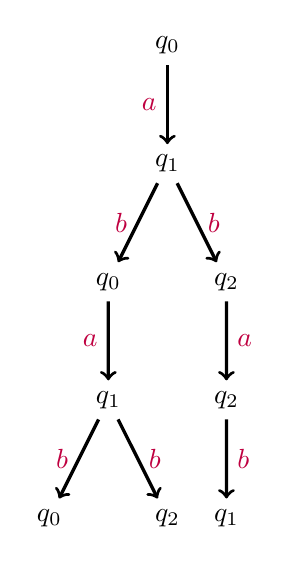
\begin{tikzpicture}
			\node {$q_0$}
			child { node {$q_1$} 
						child {node {$q_0$}
							child {node {$q_1$}
								child {node {$q_0$}
									edge from parent [->] node [left, purple] {$b$}
								}
								child {node {$q_2$}
									edge from parent [->] node [right, purple] {$b$}
								}
								edge from parent [->] node [left, purple] {$a$}
							}
							edge from parent [->] node [left, purple] {$b$}
						}
						child {node {$q_2$}
							child {node {$q_2$}
								child {node {$q_1$}
									edge from parent [->] node [right, purple] {$b$}
								}
								edge from parent [->] node [right, purple] {$a$}
							}
							edge from parent [->] node [right, purple] {$b$}
						}
						edge from parent [->] node [left, purple] {$a$}
			}
			;
		\end{tikzpicture}
		\caption{Árvore de computação da palavra ``$abab$'' no AFN da Figura \ref{fig:AFN1}.}
		\label{fig:ArvoreComputacaoAFN}
	\end{figure}
\end{exem}

Pode-se agora apresentar a noção de aceitação (reconhecimento ou computação) de palavras nos AFD.

\begin{definition}[Reconhecimento de palavras em AFN]\label{defi:PalavraAceitaPorAFN}
	Sejam $A = \langle Q, \Sigma, \delta_N, q_0, F\rangle$ um AFN e seja $w \in \Sigma^*$. A palavra $w$ é dita aceita (reconhece ou computada) por $A$ sempre que $\widehat{\delta}(q_0, w) \cap F \neq \emptyset$ e é rejeitada por $A$ em qualquer outro caso.
\end{definition}

Note que a Definição \ref{defi:PalavraAceitaPorAFN} pode ser informalmente interpretada da seguinte forma, uma palavra é aceita por um AFN $A$ se existe pelo menos um caminho de computação para $w$ que termine em um estado final, isto é, pelo menos uma das folhas na árvore de computação deve ser um estado $q \in F$, neste caso $w$ é aceita por $A$.

\begin{exem}\label{exe:AceitacaoEmAFN}
	Considerando o AFN representado pela Figura \ref{fig:AFN2} a seguir e as palavras ``$aabbbba$'' e ``$aabb$'' tem-se que: 
	$$\widehat{\delta_N}(q_0, aabbbba) = \{q_1, q_3\}$$ 
	e  
	$$\widehat{\delta_N}(q_0, aabb) = \{q_2, q_3\}$$ 
	logo a palavra ``$aabbbba$'' é aceita por tal AFN. Por outro lado, a palavra ``$aabb$'' não é aceita pelo AFN.
	
	\begin{figure}[h]
		\centering
		\begin{tikzpicture}[>=stealth, shorten >=1pt, node distance=3.0cm, on grid, auto, state/.append style={minimum size=3em}, thick ]
			\node[state, initial]				(A)               	{$q_0$};
			\node[state, accepting]				(B) [right of=A] 	{$q_1$};
			\node[state]				        (C) [right of=B] 	{$q_2$};
			\node[state]				        (D) [right of=C] 	{$q_3$};
			\path[->] (A) +(-1,0) edge (A)
			
			%Transições:
			%(Partida) edge [tipo da seta] node {simbolo lido} (Destino)
			(A) edge 			 				node [below] {$a$}		 (B)
			(A) edge [loop above]  				node 		 {$a$}		 ( )
			(B) edge 			  				node [above] {$b$}		 (C)
			(C) edge [loop above]  				node 		 {$b$}		 ( )
			(C) edge 			  				node [above] {$b$}		 (D)
			(D) edge [loop above]  				node 		 {$a$}		 ( )
			(D) edge [bend left]  				node [below] {$a$}		 (B);
		\end{tikzpicture}
		\caption{Grafo de transição de um AFN.}
		\label{fig:AFN2}
	\end{figure}
\end{exem}

Usando a definição apresentada anteriormente de palavra aceita pode-se finalmente introduzir formalmente a noção de linguagem aceita (computada ou reconhecida) pelos AFN.

\begin{definition}[Linguagem de um AFN]\label{def:LinguagemAFN}
	Seja $A = \langle Q, \Sigma, \delta_N, q_0, F\rangle$ um AFN a linguagem reconhecida (ou computada) por $A$, denotada por $\mathcal{L}(A)$, corresponde ao conjunto de todas as palavras aceitas por $A$, formalmente tem-se que:
	\begin{eqnarray}
		\mathcal{L}(A) = \{w \in \Sigma^* \mid \widehat{\delta_N}(q_0, w) \cap F \neq \emptyset\}
	\end{eqnarray}
\end{definition}

De forma similar ao que ocorre com os AFD, para mostrar que uma linguagem $L$ é aceita por algum AFN $A$ deve-se provar a igualdade $L = \mathcal{L}(A)$, ou seja, deve-se provar que $w \in L \Longleftrightarrow w \in \mathcal{L}(A)$.

\begin{exem}\label{exe:LinguagemAFN1}
	A linguagem $L = \{a^i(ba)^j \mid i \geq 1,j \geq 0\}$ é aceita pelo AFN $A$ representado pelo grafo de transição da Figura \ref{fig:AFN3} a seguir.
	
	\begin{figure}[h]
		\centering
		\begin{tikzpicture}[>=stealth, shorten >=1pt, node distance=3.0cm, on grid, auto, state/.append style={minimum size=3em}, thick ]
			\node[state, initial]				(A)               	{$s_0$};
			\node[state, accepting]				(B) [right of=A] 	{$s_1$};
			\node[state]				        (C) [right of=B] 	{$s_2$};
			\path[->] (A) +(-1,0) edge (A)
			
			%Transições:
			%(Partida) edge [tipo da seta] node {simbolo lido} (Destino)
			(A) edge [loop above]  				node 		 {$a$}		 ( )
			(A) edge 			  				node 		 {$a$}		 (B)
			(B) edge [bend left]  				node 		 {$b$}		 (C)
			(C) edge [bend left]  				node 		 {$a$}		 (B);
		\end{tikzpicture}
		\caption{Grafo de transição de um AFN.}
		\label{fig:AFN3}
	\end{figure}

	\begin{proof}
		$(\Rightarrow)$ Suponha que $w \in L$, portanto, $w = a^m(ba)^n$,  e agora por indução dupla sobre o par $(m,n)$ tem-se que:
		
		\begin{itemize}
			\item \textbf{Base da indução}:
			
			Quando com $m = 1$ e $n = 0$ vale a igualdade $w = a^1(ba)^0 = a$, agora usando a definição de $\delta_N$ do AFN $A$ como representado na Figura \ref{fig:AFN3} tem-se que, 
			\begin{eqnarray*}
				\widehat{\delta_N}(s_0, a) = \bigcup_{s' \in \widehat{\delta}(s_0, \lambda)} \delta_N(s', a) = \delta_N(s_0, a) = \{s_0, s_1\}
			\end{eqnarray*}
			uma vez que, $s_1 \in F$ tem-se que $\widehat{\delta_N}(s_0, a) \cap F \neq \emptyset$, e portanto, $w \in \mathcal{L}(A)$. Agora suponha que para $w = a^1(ba)^n$ com $n \geq 0$ tem-se que $\widehat{\delta_N}(s_0, a^1(ba)^n) \cap F \neq \emptyset$. Assim dado $a^1(ba)^{n+1}$ por definição tem-se que:
			\begin{eqnarray}\label{eq:ProvaAFNLinguagem1}
				\widehat{\delta_N}(s_0, a^1(ba)^{n+1}) & = & \widehat{\delta_N}(s_0, a^1(ba)^{n}ba)\nonumber\\
				& = & \bigcup_{s' \in \widehat{\delta_N}(s_0, a^1(ba)^{n}b)} \delta_N(s', a)
			\end{eqnarray}
			agora fazendo,
			\begin{eqnarray}\label{eq:ProvaAFNLinguagem2}
				K = \bigcup_{s'' \in \widehat{\delta_N}(s_0, a^1(ba)^{n})} \delta_N(s'', b)
			\end{eqnarray}
			e reescrevendo a Equação (\ref{eq:ProvaAFNLinguagem1}) usando a Equação (\ref{eq:ProvaAFNLinguagem2}) tem-se que,
			\begin{eqnarray}\label{eq:ProvaAFNLinguagem3}
				\widehat{\delta_N}(s_0, a^1(ba)^{n+1}) & = & \bigcup_{s' \in K} \delta_N(s', a)
			\end{eqnarray}
			entretanto, por hipótese tem-se que $\widehat{\delta_N}(s_0, a^1(ba)^n) \cap F \neq \emptyset$, consequentemente, tem-se que $s_1 \in \widehat{\delta_N}(s_0, a^1(ba)^n)$ dessa forma pela Equação (\ref{eq:ProvaAFNLinguagem2}) é claro que $\delta_N(s_1, b) \subseteq K$. Mas $\delta_N(s_1, b) = \{s_2\}$ logo pela Equação (\ref{eq:ProvaAFNLinguagem3}) tem-se que $\delta_N(s_2, a) \subseteq \widehat{\delta_N}(s_0, a^1(ba)^{n+1})$, desde que $\delta_N(s_2, a) = \{s_1\}$, tem-se $s_1 \in \widehat{\delta_N}(s_0, a^1(ba)^{n+1})$, portanto, $\widehat{\delta_N}(s_0, a^1(ba)^{n+1}) \cap F \neq \emptyset$, consequentemente $a^1(ba)^{n+1} \in \mathcal{L}(A)$.
			\item \textbf{Hipótese indutiva (HI)}:
			
			Assuma que para todo $n \geq 0$ tem-se que $\widehat{\delta_N}(s_0, a^m(ba)^n)  \cap F \neq \emptyset$.
			\item \textbf{Passo indutivo}:
			
			Primeiro seja $w \in L$ de forma que $w = a^{m+1}(ba)^0$ logo pela hipótese indutiva segue que, 
			\begin{eqnarray*}
				\widehat{\delta_N}(s_0, a^{m+1}(ba)^0) \cap F \neq \emptyset
			\end{eqnarray*}
			consequentemente, $a^{m+1}(ba)^0 \in \mathcal{L}(A)$. Por outro lado, sendo $w \in L$ tal que $w = a^{m+1}(ba)^n$, usando a  definição de $\widehat{\delta_N}$ tem-se para $a^{m+1}(ba)^{n+1}$ que, 
			\begin{eqnarray}\label{eq:ProvaAFNLinguagem4}
				\widehat{\delta_N}(s_0, a^{m+1}(ba)^{n+1}) & = & \widehat{\delta_N}(s_0, a^{m+1}(ba)^{n}ba)\nonumber\\
				& = & \bigcup_{s' \in \widehat{\delta_N}(s_0, a^{m+1}(ba)^{n}b)} \delta_N(s', a)
			\end{eqnarray}
			agora desenvolvendo o termo $\widehat{\delta_N}(s_0, a^{m+1}(ba)^{n}b)$ tem-se
			\begin{eqnarray*}
				\widehat{\delta_N}(s_0, a^{m+1}(ba)^{n}b) & = & \bigcup_{s'' \in \widehat{\delta_N}(s_0, a^{m+1}(ba)^{n})} \delta_N(s'', b)
			\end{eqnarray*}
			pela hipótese indutiva tem-se que $\widehat{\delta_N}(s_0, a^{m+1}(ba)^{n}) \cap F = \emptyset$, consequentemente, $s_1 \in \widehat{\delta_N}(s_0, a^{m+1}(ba)^{n})$, logo $\delta_N(s_1, b) \subseteq \widehat{\delta_N}(s_0, a^{m+1}(ba)^{n})$, uma vez que, $\delta_N(s_1, b) = \{s_2\}$, tem-se que $\{s_2\} \subseteq \widehat{\delta_N}(s_0, a^{m+1}(ba)^{n})$, assim pela Equação (\ref{eq:ProvaAFNLinguagem4}) segue que $\delta_N(s_2, a) \subseteq \widehat{\delta_N}(s_0, a^{m+1}(ba)^{n+1})$, mas por definição $\delta_N(s_2, a) = \{s_1\}$, portanto, tem-se que $\{s_1\} \subseteq \widehat{\delta_N}(s_0, a^{m+1}(ba)^{n+1})$, logo $\widehat{\delta_N}(s_0, a^{m+1}(ba)^{n+1}) \cap F \neq \emptyset$ e assim $a^{m+1}(ba)^{n+1} \in \mathcal{L}(A)$.
		\end{itemize}
		$(\Leftarrow)$ Suponha que $w \in \mathcal{L}(A)$ assim $s_1 \in \widehat{\delta_N}(s_0, w)$, note porém que $s_1$ só é acessível a partir de duas transições: 
		\begin{itemize}
			\item (1) $\delta_N(s_0, a)$ e
			\item (2) $\delta_N(s_2, a)$. 
		\end{itemize}
		Note que devido ao \textit{loop} fornecido pelo fato de que $s_0 \in \delta_N(s_0, a)$ a transição (1) pode ser executada $m$ vezes com $m \geq 1$, em que para cada execução um novo ramo com o estado $s_1$ é gerado na árvore de computação de $A$, entretanto, executar $m$ vezes a transição $\delta_N(s_0, a)$ implica em executar a computação $\widehat{\delta_N}(s_0, a^m)$, pelo fato\footnote{Fica para o leitor a tarefa de provar que para todo $m \geq 1$ tem-se que $s_1 \in \widehat{\delta_N}(s_0, a^m)$.} de que $s_1 \in \widehat{\delta_N}(s_0, a^m)$ tem-se que $a^m \in \mathcal{L}(A)$, e uma vez que $a^m = a^m(ba)^0$ tem-se que a primeira forma de $\widehat{\delta_N}(s_0, w) \cap F \neq \emptyset$ é que $w = a^m(ba)^0$ e assim $w \in L$. Por outro lado, para acessar $s_1$ via a transição (2) é necessário antes chegar a um ramo de computação em que o estado $s_2$ seja uma folha, mas pela definição de $A$ isso só é possível se a transição $\delta_N(s_1, b)$ for usada, note entretanto, que as transições $\delta_N(s_1, b) = \{s_2\}$ e $\widehat{\delta_N}(s_2, a) = \{s_1\}$ também geram um \textit{loop} que pode ser executado $n$ vezes com $n \geq 0$, mas executar esse \textit{loop} $n$ vezes corresponde a executar $\widehat{\delta_N}(s_1, (ba)^n)$, e como dito anteriormente, $s_1$ só é acessível pela definição de $A$ usando a computação $\widehat{\delta_N}(s_0, a^m)$, portanto, para que $s_1 \in \widehat{\delta_N}(s_0, w) \cap F$, obrigatoriamente, $w = a^m(ba)^n$ com $m \geq 1, n \geq 0$, e portanto, $w \in L$.
	\end{proof}
\end{exem}

\begin{exem}\label{exe:LinguagemAFN2}
	O AFN $S$ representado no grafo de transição exposto na Figura \ref{fig:AFN4} a seguir reconhece a linguagem $L = \{uv \mid u \in \{0,1\}^*,  v \in \{0,1\}\}$.
	
	\begin{figure}[h]
		\centering
		\begin{tikzpicture}[>=stealth, shorten >=1pt, node distance=3.0cm, on grid, auto, state/.append style={minimum size=3em}, thick ]
			\node[state, initial]						(A)               	{$s_0$};
			\node										(B) [right of=A] 	{ };
			\node[state, accepting]				        (C) [above of=B] 	{$s_1$};
			\node[state, accepting]				        (D) [below of=B] 	{$s_2$};
			\path[->] (A) +(-1,0) edge (A)
			
			%Transições:
			%(Partida) edge [tipo da seta] node {simbolo lido} (Destino)
			(A) edge [loop above]  				node 		 {$0, 1$}		 ( )
			(A) edge							node 		 {$0$}			 (C)
			(A) edge							node 		 {$1$}			 (D);
		\end{tikzpicture}
		\caption{Grafo de transição de um AFN $S$.}
		\label{fig:AFN4}
	\end{figure}

	\begin{proof}
		$(\Rightarrow)$ A ida fica a cargo do leitor. $(\Leftarrow)$ Suponha que $w \in \mathcal{L}(A)$ assim por definição $\widehat{\delta_N}(s_0, w) \cap \{s_1, s_2\} \neq \emptyset$, agora pela definição de $\delta_N$ é claro que toda árvore de computação de $A$ apresenta a propriedade de sempre conter um dos estados $s_1$ ou $s_2$, mas nunca os dois simultaneamente\footnote{A prova desta propriedade fica como exercício ao leitor.}, além disso, o fato de $s_0 \in \widehat{\delta_N}(s_0, a)$ para todo $a \in \{0,1\}$, garante que qualquer palavra não a vazia $u$ sobre o alfabeto $\{0,1\}$ pode ser gerada, por fim, no último passo de computação é claro que $s_1$ ou $s_2$ será uma folha da árvore, entretanto, $s_1$ só será tal folha no caso da palavra terminar em $0$ caso contrário a folha será $s_2$, e portanto, todo $w \in \mathcal{L}(A)$ tem a foma $uv$ com $u \in \{0, 1\}^*$ e $v \in \{0,1\}$, consequentemente $w \in L$.
	\end{proof}
\end{exem}

De forma ingênua o leitor pode vim a imaginar que a possibilidade da unidade de controle de um AFN poder assumir mais de um estado interno simultaneamente, faz com que os AFN sejam mais poderosos que os AFD, entretanto, como será exibido pelos resultados a seguir, isso não ocorre, de fato, como dito \cite{benjaLivro2010, linz2006} apesar de tornar mais fácil a tarefa de construir um autômato quem reconheça uma linguagem $L$, o não-determinismo não aumenta nem nada o poder de computação dos autômatos finitos.

\begin{theorem}[Transformação AFD - AFN]\label{teo:AFD-Para-AFN}
	Se $L = \mathcal{L}(A)$ para algum AFD $A$, então existe um AFN $A'$ tal que $L = \mathcal{L}(A')$.
\end{theorem}

\begin{proof}
	A prova é trivial, uma vez que, todo AFD $A = \langle Q, \Sigma, \delta, q_0, F\rangle$ pode ser convertido em um AFN $A' = \langle Q, \Sigma, \delta_N, q_0, F\rangle$ apenas realizando as transformações das transições $\delta(q_i, a) = q_j$ nas transições não-determinísticas $\delta_N(q_i, a) = \{q_j\}$ e mantendo todo o resto da estrutura igual.
\end{proof}

O próximo resultado estabelece a contraparte do Teorema \ref{teo:AFD-Para-AFN}, isto é, tal resultado mostrará que sempre é possível obter um AFD que pode ``simular''\footnote{Um termo simular aqui, diz respeito a ideia de que cada aplicação de um função de transição não-determinística pode ser representada de forma precisa por uma aplicação de uma função de transição determinística, para detalhes consulte \cite{hopcroft2008, menezes1998LFA}.} um AFN.

\begin{theorem}[Transformação AFN - AFD]\label{teo:AFN-Para-AFD}
	Se $L = \mathcal{L}(A)$ para algum AFN $A$, então existe um AFD $A'$ tal que $L = \mathcal{L}(A')$.
\end{theorem}

\begin{proof}
	Suponha que $L = \mathcal{L}(A)$ para algum AFN $A = \langle Q, \Sigma, \delta_N, q_0, F\rangle$, agora é construído um  autômato $A' = \langle \wp(Q), \Sigma, \delta, \{q_0\}, F' \rangle$ onde para todo $X \in \wp(Q)$ e $a \in \Sigma$ tem-se
	\begin{eqnarray}\label{eq:TranformacaoDelta-DeltaN}
		\delta(X, a) = \bigcup_{q \in X} \delta_N(q, a)
	\end{eqnarray}
	claramente este autômato é realmente determinístico, e para todo $X \in \wp(Q)$  tem-se que $X \in F'$ se, e somente se, $X \cap F \neq \emptyset$. Agora será mostrado por indução sobre o tamanho de $w \in \Sigma^*$ que:
	$$\widehat{\delta}(\{q_0\}, w) = \widehat{\delta_N}(q_0, w)$$
	\begin{itemize}
		\item \textbf{Base da indução}:
		
		Quando $|w| = 0$ isto é $w = \lambda$ tem-se trivialmente pela definição das funções de transição estendidas que $\widehat{\delta}(\{q_0\}, \lambda) = \widehat{\delta_N}(q_0, \lambda)$.
		
		\item \textbf{Hipótese indutiva (HI)}:
		
		Suponha que para todo $w \in \Sigma^*$ com $|w| \geq 0$ tem-se que $\widehat{\delta}(\{q_0\}, w) = \widehat{\delta_N}(q_0, w)$.
		\item \textbf{Passo indutivo}:
		
		Dado $w = ua$ com $u \in \Sigma^*$, $|u| \geq 0$ e $a \in \Sigma$ tem-se que, 
		\begin{eqnarray*}
			\widehat{\delta}(\{q_0\}, w) & = & \widehat{\delta}(\{q_0\}, ua)\\
			& = & \delta(\widehat{\delta}(\{q_0\}, u), a)\\
			& \stackrel{\textbf{(HI)}}{=} & \delta(\widehat{\delta_N}(q_0, u), a)\\
			& \stackrel{Eq. (\ref{eq:TranformacaoDelta-DeltaN})}{=} & \bigcup_{q \in \widehat{\delta_N}(q_0, u)} \delta_N(q, a)\\
			& = & \widehat{\delta_N}(q_0, ua)\\
			& = & \widehat{\delta_N}(q_0, w)
		\end{eqnarray*}
	\end{itemize}
	Portanto, pode-se concluir que $w \in \mathcal{L}(A)$ se, e somente se, $w \in \mathcal{L}(A')$, ou seja, $L = \mathcal{L}(A')$ o que completa a prova.
\end{proof}

Observe que o método de construção usado na prova do Teorema \ref{teo:AFN-Para-AFD} cria um AFD cujo número de estado cresce em razão de uma potência de 2 quando comparado com o quantitativo de estados do AFN original. Como consequência deste resultado segue o seguinte corolário.

\begin{corollary}
	Uma linguagem $L$ é regular se, e somente se, existe um AFN $A$ tal que $L = \mathcal{L}(A)$.
\end{corollary}

\begin{proof}
	$(\Rightarrow)$ Assuma que $L$ é regular, assim por definição existe um AFD $A'$ tal que $L = \mathcal{L}(A')$, entretanto, pelo Teorema \ref{teo:AFD-Para-AFN} existe um AFN $A$ tal que $L = \mathcal{L}(A)$. $(\Leftarrow)$ Suponha que $L = \mathcal{L}(A)$ para algum AFN $A$, agora pelo Teorema \ref{teo:AFN-Para-AFD} existe um AFD $A'$ tal que $L = \mathcal{L}(A')$, e portanto, por definição $L$ é regular.
\end{proof}

\

É importante destacar que o método de construção do AFD usado na prova do Teorema \ref{teo:AFN-Para-AFD}, conhecido como método de construção das partes introduzido por Rabin e Scott em \cite{rabin1959}, tem a característica de poder vim a produzir durante sua execução alguns estados inacessíveis\footnote{Um estado $q$ em um AFD é dito inacessível se não existe um $w \in \Sigma^*$ tal que $\widehat{\delta}(q_0, w) = q$. Vale também ressaltar como destaco em \cite{benjaLivro2010, hopcroft2008} que estados inacessíveis não aumentam o poder de computação nos AFD.} no AFD resultante, além disso,  o método de construção das partes em alguns cenários pode ser tornar impraticável, pois se o AFN de entrada possuir $n$ estados, o AFD resultante do método terá $2^n$ estados, ou seja, o crescimento no número de estados do AFD resultante do método cresce proposicional a uma potência de 2, o que rapidamente gera um número exponencialmente grande de estados. 

A seguir o leitor será apresentado a uma melhoria no algoritmo de construção das partes, no sentido de que, a execução de tal algoritmo não produz estados inacessíveis no AFD de saída, o algoritmo a seguir é um pseudo-código baseado na versão textual apresentada no livro de por Bedregal \textit{et al.} \cite{benjaLivro2010}. A melhoria no Algoritmo \ref{alg:AFN-AFD} consiste do fato dele não considerar simplesmente o conjunto $\wp(Q)$ no AFD de saída, em vez disso, ele constrói interativamente um conjunto de estados $Q' \subseteq \wp(Q)$, que no pior caso\footnote{A expressão ``no pior caso'' é típica da análise de algoritmos, em momentos futuros essa ideia de pior caso será melhor desenvolvida neste manuscrito.} $Q' = \wp(Q)$.

\begin{algorithm}[h]
	\Entrada{Um AFN $A = \langle Q, \Sigma, \delta_N, q_0, F\rangle$}
	\Saida{Um AFD $A' = \langle Q', \Sigma, \delta, \{q_0\}, F' \rangle$}
	\Inicio{
		Inicialize o conjuntos $Q_u$ com um  estado rotulado por $\{q_0\}$\\
		Inicialize o conjuntos $Q'$ com um  estado rotulado por $\{q_0\}$\\
		Inicialize o conjunto $F'$ como sendo vazio\\
		\Repita{$Q_u = \emptyset$}{
			Selecione um estado $X \in Q_u$\\
			\ParaCada{$a \in \Sigma$}{
				Determine o conjunto $\displaystyle Y = \bigcup_{q \in X}\delta_N(q, a)$\\
				\eSe{$Y \notin Q'$}{
					Adicione um estado rotulado por $Y$ em $Q'$\\
					Adicione um estado rotulado por $Y$ em $Q_u$\\
					Defina a transição $\delta(X, a) = Y$\\
				}{
					Defina a transição $\delta(X, a) = Y$\\
				}
			}
			Remova $X$ de $Q_u$
		}
		\ParaCada{$X \in Q'$}{
			\Se{$X \cap F \neq \emptyset$}{
				Adicione $X$ ao conjunto $F'$
			}
		}
		\Retorna{$A' = \langle Q', \Sigma, \delta, \{q_0\}, F' \rangle$}
	}
	\caption{Algoritmo para converter AFN em AFD sem estados inacessíveis.}
	\label{alg:AFN-AFD}
\end{algorithm}

\begin{exem}\label{exe:ConvertendoAFN-AFD}
	Usando o Algoritmo \ref{alg:AFN-AFD}  no AFN representado pelo grafo de transição da Figura \ref{fig:AFN2} é obtido o AFD representado no grafo de transição da Figura \ref{fig:AFN-AFD1} exposta a seguir.
\end{exem}

\begin{figure}[h]
	\centering
	\begin{tikzpicture}[>=stealth, shorten >=1pt, node distance=3.0cm, on grid, auto, state/.append style={minimum size=3em}, thick ]
		\node[state, initial]				(A)               	{$\{q_0\}$};
		\node[state, accepting]				(B) [right of=A] 	{$\{q_0, q_1\}$};
		\node[state]				        (C) [right of=B] 	{$\{q_2\}$};
		\node[state]				        (D) [right of=C] 	{$\{q_2, q_3\}$};
		\node[state, accepting]				(E) [below of=D] 	{$\{q_1, q_3\}$};
		\node[state]				        (F) [below of=B] 	{$\emptyset$};
		\path[->] (A) +(-1,0) edge (A)
		
		%Transições:
		%(Partida) edge [tipo da seta] node {simbolo lido} (Destino)
		(A) edge 			 				node		 {$a$}		 (B)
		(A) edge 			 				node  		 {$b$}		 (F)
		(B) edge [loop below] 				node 		 {$a$}		 ( )
		(B) edge 			 				node  		 {$b$}		 (C)
		(C) edge 			 				node  		 {$a$}		 (F)
		(C) edge 			 				node  		 {$b$}		 (D)
		(D) edge 			 				node  		 {$a$}		 (E)
		(D) edge [loop right] 				node  		 {$b$}		 ( )
		(E) edge [loop right] 				node  		 {$a$}	 	 ( )
		(E) edge 			 				node  		 {$b$}		 (C)
		(F) edge [loop left] 				node  		 {$a,b$}	 ( );
	\end{tikzpicture}
	\caption{Grafo de transição de um AFD equivalente ao AFN da Figura \ref{fig:AFN2}.}
	\label{fig:AFN-AFD1}
\end{figure}

\subsection{$\lambda$-Autômatos Finitos Não-determinísticos}\label{subsec:LAFN}

Os $\lambda$-Autômatos Finitos Não-determinísticos, ou simplesmente, $\lambda$-AFN são como dito em \cite{menezes1998LFA}, uma generalização do modelo de AFN  introduzido na seção anterior e que são permitidas transições entre estados diferentes usando (ou consumindo) a palavra vazia, tais transições recebem o nome de $\lambda$-transições, a seguir tais autômatos serão apresentados formalmente.

\begin{definition}[$\lambda$-Autômatos Finitos Não-determinísticos]\label{def:LAFN}
	Um $\lambda$-AFN é uma estrutura $A = \langle Q, \Sigma, \underline{\delta_N}, q_0, F\rangle$ onde: $Q, \Sigma, q_0$ e $F$ são da mesma forma que na Definição \ref{def:AFD}, já $\underline{\delta_N} : Q \times (\Sigma \cup \{\lambda\}) \rightarrow \wp(Q)$ é uma função total (chamada $\lambda$-função de transição não determinística).
\end{definition}

A representação usando grafos de transição dos $\lambda$-AFN e similar a representação dos AFN da seção anterior, a única diferença é que podem haver transições rotuladas pelo símbolo $\lambda$, isto é, podem existir no grafo arestas entre vértices que são rotuladas por $\lambda$, e o mesmo vale para a representação das árvores de computação.

\begin{exem}\label{exe:LAFN1}
	A estrutura $A = \langle \{q_0, q_1, q_2\}, \{0,1\}, \underline{\delta_N}, q_0, \{q_0\}\rangle$ com $\underline{\delta_N}$ sendo especificada pela Tabela \ref{tab:DeltaLAFN1} a seguir é um $\lambda$-AFN.
	
	\begin{table}[h]
		\centering
		\begin{tabular}{c|ccc}
			\backslashbox{$Q$}{$\Sigma \cup \{\lambda\}$}	& $0$ & $1$ & $\lambda$\\ \hline
			$q_0$  & $\emptyset$ & $\emptyset$ & $\{q_1\}$\\
			$q_1$  & $\{q_1\}$ & $\{q_2\}$ & $\{q_2\}$\\
			$q_2$  & $\{q_2\}$ & $\{q_2\}$ & $\{q_0, q_2\}$ \\
		\end{tabular}
		\caption{Tabela de transição para a função $\delta_N$ do AFN no Exemplo \ref{exe:LAFN1}.}
		\label{tab:DeltaLAFN1}
	\end{table}
\end{exem} 

\begin{rema}
	Uma interpretação para as transições da forma $\underline{\delta_N}(q, \lambda) = X$ é que a unidade de controle do autômato consegue mudar seu estado interno $q$ para um subconjunto de estados $X$ sem precisar acessar a memória.
\end{rema}

\begin{exem}
	O grafo de transição representado na Figura \ref{fig:LAFN1} a seguir é uma representação para o $\lambda$-AFN do Exemplo \ref{exe:LAFN1}.
	
	\begin{figure}[h]
		\centering
		\begin{tikzpicture}[>=stealth, shorten >=1pt, node distance=2.5cm, on grid, auto, state/.append style={minimum size=3em}, thick ]
			\node[state, initial, accepting]	(A)               	{$q_0$};
			\node[state, accepting]				(B) [right of=A] 	{$q_1$};
			\node[state]				        (C) [right of=B] 	{$q_2$};
			\path[->] (A) +(-1,0) edge (A)
			
			%Transições:
			%(Partida) edge [tipo da seta] node {simbolo lido} (Destino)
			(A) edge							node 		 {$\lambda$} (B)
			(B) edge							node [above] {$1, \lambda$} (C)
			(B) edge [loop above]  				node 		 {$0$} 		 ( )
			(C) edge [loop above]  				node 		 {$1, 0, \lambda$} ( )
			(C) edge [bend left]  				node [below] {$\lambda$} (A);
		\end{tikzpicture}
		\caption{Grafo de transição do $\lambda$-AFN do Exemplo \ref{exe:LAFN1}.}
		\label{fig:LAFN1}
	\end{figure}
\end{exem}

Note porém que a definição da função de transição $\underline{\delta_N}$ garante que as transições em um $\lambda$-AFN acontece apenas em duas situações, a primeira em relação símbolos individuais do alfabeto $\Sigma$ e a segunda com relação a palavra vazia, assim não existe uma forma de computar uma palavra $w$ de forma que $|w| > 1$. A saída para contorna esse fato é estender a função de transição do autômato, similarmente ao que é feito para os AFD e AFN, para isso entretanto, é necessária algumas definições adicionais.

\begin{definition}[Função $\delta_\lambda$]\label{def:L-fecho}
	Seja $A = \langle Q, \Sigma, \underline{\delta_N}, q_0, F\rangle$ um $\lambda$-AFN, então a função $\delta_\lambda: Q \rightarrow \wp(Q)$ é definida como,
	\begin{equation}
		\delta_\lambda(q) = \bigcup_{i = 0}^n\lambda\text{-fecho}^i(q)
	\end{equation}
	onde $n = \# Q - 1$ e
	\begin{eqnarray}
		\lambda\text{-fecho}^0(q) & = & \{q\}\\
		\lambda\text{-fecho}^{i}(q) & = & \bigcup_{q' \in \lambda\text{-fecho}^{i-1}(q)} \delta_N(q', \lambda)
	\end{eqnarray}
\end{definition}

\begin{exem}
	Considere o $\lambda$-AFN da Figura \ref{fig:LAFN1} tem-se para o estado $q_0$ que,
	\begin{eqnarray}\label{eq:LAFNeq1}
		\lambda\text{-fecho}^{2}(q_1) & = &  \bigcup_{q' \in \lambda\text{-fecho}^{1}(q_1)} \delta_N(q', \lambda)
	\end{eqnarray}
	desenvolvendo $q' \in \lambda\text{-fecho}^{1}(q_0)$ tem-se que,
	\begin{eqnarray*}
		\lambda\text{-fecho}^{1}(q_1) & = &  \bigcup_{q' \in \lambda\text{-fecho}^{0}(q_1)} \delta_N(q', \lambda)
	\end{eqnarray*}
	mas, 
	\begin{eqnarray*}
		\lambda\text{-fecho}^{0}(q_1) & = & \{q_1\}
	\end{eqnarray*}
	assim, 
	\begin{eqnarray*}
		\lambda\text{-fecho}^{1}(q_1) & = &  \{q_2\}
	\end{eqnarray*}
	substituindo tal resultado na Equação \ref{eq:LAFNeq1} tem-se que, 
	\begin{eqnarray*}\label{eq:LAFNeq2}
		\lambda\text{-fecho}^{2}(q_1) & = & \bigcup_{q' \in \{q_2\}} \delta_N(q', \lambda)\\
		& = & \{q_2, q_0\}
	\end{eqnarray*}
	logo $\delta_\lambda(q_1) = \{q_0, q_1, q_2\}$.
\end{exem}

Uma interpretação semântica para a função $\delta_\lambda$ é que ela representa a resposta ao questionamento: ``Estando no estado $q$ e executando $n$ $\lambda$-transições qual subconjunto de estados a unidade central do autômato irá assumir?''. Assim como acontecer com as funções de transição a função $\delta_\lambda$ pode ser estendida, a seguir é exposto tal extensão.

\begin{definition}[Função $\widehat{\delta_\lambda}$]\label{def:L-Fecho}
	Seja $A = \langle Q, \Sigma, \underline{\delta_N}, q_0, F\rangle$ um $\lambda$-AFN, então a função $\widehat{\delta_\lambda}: \wp(Q) \rightarrow \wp(Q)$ é definida como,
	\begin{equation}
		\widehat{\delta_\lambda}(X) = \bigcup_{q \in X} \delta_\lambda(q)
	\end{equation}
\end{definition} 

\begin{exem}
	Considere o $\lambda$-AFN da Figura \ref{fig:LAFN1} tem-se para o conjunto $\{q_1, q_2\}$ que,
	\begin{eqnarray*}
		\widehat{\delta_\lambda}(\{q_1, q_2\}) & = & \bigcup_{q \in \{q_1, q_2\}} \delta_\lambda(q)\\
		& = & \delta_\lambda(q_1) \cup \delta_\lambda(q_2)\\
		& = & \{q_0, q_1, q_2\} \cup \{q_0, q_2, q_1\}\\
		& = & \{q_0, q_2, q_1\}
	\end{eqnarray*}
\end{exem}

Agora usando as definições de $\delta_\lambda$ e $\widehat{\delta_\lambda}$ pode-se apresentar a extensão da função de transição dos $\lambda$-AFN.

\begin{definition}[$\lambda$-Transição não-determinística estendida]\label{def:FuncaoLDeltaNDEstendida}
	Seja $A = \langle Q, \Sigma, \underline{\delta_N}, q_0, F\rangle$  um $\lambda$-AFN a função $\underline{\delta_N}$ é estendido para a função $\widehat{\underline{\delta_N}}: Q \times \Sigma^* \rightarrow \wp(Q)$ definida pela seguinte recursão:
	\begin{eqnarray}\label{eq:FuncaoLDeltaNDEstendida}
		\widehat{\underline{\delta_N}}(q, \lambda)& = &  \delta_\lambda(q)\\
		\widehat{\underline{\delta_N}}(q, wa) & = & \bigcup_{q' \in \widehat{\underline{\delta_N}}(q, w)} \widehat{\delta_\lambda}(\underline{\delta_N}(q', a))
	\end{eqnarray}
\end{definition}

\begin{exem}
	Considere o $\lambda$-AFN da Figura \ref{fig:LAFN1} tem-se a seguinte computação para a palavra $``10''$:
	\begin{eqnarray}\label{eq:ExemLAFN1}
		\widehat{\underline{\delta_N}}(q_0, 10) & = & \bigcup_{q' \in \widehat{\underline{\delta_N}}(q_0, 1)} \widehat{\delta_\lambda}(\underline{\delta_N}(q', 0))\nonumber\\
		& = & \bigcup_{q' \in \widehat{\underline{\delta_N}}(q_0, 1)} \widehat{\delta_\lambda}(\underline{\delta_N}(q', 0))
	\end{eqnarray}
	mas,
	\begin{eqnarray}\label{eq:ExemLAFN2}
		\widehat{\underline{\delta_N}}(q_0, 1) & = & \bigcup_{q' \in \widehat{\underline{\delta_N}}(q_0, \lambda)} \widehat{\delta_\lambda}(\underline{\delta_N}(q', 1))\nonumber\\
		& = & \bigcup_{q' \in \delta_\lambda(q_0)} \widehat{\delta_\lambda}(\underline{\delta_N}(q', 1))\nonumber\\
		& = & \bigcup_{q' \in \{q_0, q_1, q_2\}} \widehat{\delta_\lambda}(\underline{\delta_N}(q', 1))\\
		& = & \widehat{\delta_\lambda}(\{q_1, q_2\})\nonumber\\
		& = & \{q_0, q_1, q_2\}\nonumber
	\end{eqnarray}
	substituindo o valor da Equação (\ref{eq:ExemLAFN2}) na Equação (\ref{eq:ExemLAFN1}) tem-se que, 
	\begin{eqnarray*}
		\widehat{\underline{\delta_N}}(q_0, 10) & = & \bigcup_{q' \in \{q_0, q_1, q_2\}} \widehat{\delta_\lambda}(\underline{\delta_N}(q', 0))\\
		& = & \{q_0, q_1, q_2\}
	\end{eqnarray*}
\end{exem}

Assim como para o caso dos AFN uma palavra qualquer $w \in \Sigma^*$ será dita aceita por um $\lambda$-AFN quando a computação da palavra $w$ para em pelo menos um estado final, ou seja, $w$ é reconhecida pelo $\lambda$-AFN sempre que $\widehat{\underline{\delta_N}}(q_0, w) \cap F \neq \emptyset$, e assim pode-se definir formalmente a noção de linguagem para os $\lambda$-AFN.

\begin{definition}[Linguagem de um $\lambda$-AFN]\label{def:LinguagelLAFN}
	Seja $A = \langle Q, \Sigma, \underline{\delta_N}, q_0, F\rangle$ um $\lambda$-AFN a linguagem aceita por $A$, denotado por $\mathcal{L}(A)$, corresponde ao seguinte conjunto.
	\begin{eqnarray}
		\mathcal{L}(A) = \{w \in \Sigma^* \mid \widehat{\underline{\delta_N}}(q_0, w) \cap F \neq \emptyset\}
	\end{eqnarray}
\end{definition}

Os aspectos relacionados a mostrar que um $\lambda$-AFN reconhece uma linguagem $L$ são similares ao mesmo aspectos com respeito aos AFN.

\begin{exem}\label{exe:LinguagemLAFN1}
	O $\lambda$-AFN representado pelo grafo de transição da Figura \ref{fig:Linguagem-LAFN1} a seguir reconhece a linguagem $L = \{w \in \{1,2,3\}^* \mid w = 1^i2^j3^k \text{ com } i,j,k \in \mathbb{N}\}$.
	
	\begin{figure}[h]
		\centering
		\begin{tikzpicture}[>=stealth, shorten >=1pt, node distance=3.0cm, on grid, auto, state/.append style={minimum size=3em}, thick ]
			\node[state, initial, accepting]	(A)               	{$s_0$};
			\node[state, accepting]				(B) [right of=A] 	{$s_1$};
			\node[state]				        (C) [right of=B] 	{$s_2$};
			\path[->] (A) +(-1,0) edge (A)
			
			%Transições:
			%(Partida) edge [tipo da seta] node {simbolo lido} (Destino)
			(A) edge [loop above]  				node 		 {$1$} 		 ( )
			(A) edge 			  				node 		 {$\lambda$} (B)
			(B) edge [loop above]  				node 		 {$2$} 		 ( )
			(B) edge 			  				node 		 {$\lambda$} (C)
			(C) edge [loop above]  				node 		 {$3$} 		 ( );
		\end{tikzpicture}
		\caption{Grafo de transição do $\lambda$-AFN do Exemplo \ref{exe:LinguagemLAFN1}.}
		\label{fig:Linguagem-LAFN1}
	\end{figure}
\end{exem}

\begin{figure}[h]
	\centering
	\begin{tikzpicture}[>=stealth, shorten >=1pt, node distance=2.7cm, on grid, auto, state/.append style={minimum size=3em}, thick ]
		\node[state, initial]				(A)               	{$s_0$};
		\node[state, accepting]				(B) [right of=A]	{$s_3$};
		\node[state] 						(C) [above of=B] 	{$s_1$};
		\node[state] 						(D) [below of=B] 	{$s_2$};
		\node[state]						(E) [right of=B] 	{$s_5$};
		\node[state] 						(F) [above of=E] 	{$s_4$};
		\node[state] 						(G) [right of=D] 	{$s_6$};
		
		
		\path[->] (A) +(-1,0) edge (A)
		
		%Transições:
		%(Partida) edge [tipo da seta] node {simbolo lido} (Destino)  [loop right]  
		(A) edge  							node 		 {$\lambda$}	 (C)
		(A) edge  							node 		 {$\lambda$}	 (D)
		(A) edge  							node 		 {$b$}	 		 (B)
		(B) edge [loop right]  				node 		 {$a,b$}		 ( )
		(C) edge [bend left]				node 		 {$a$}			 (F)
		(C) edge							node		 {$b$}			 (B)
		(F) edge [bend left]				node 		 {$a$}			 (C)
		(D) edge							node		 {$a$}			 (G)
		(G) edge							node		 {$a$}			 (E)
		(E) edge							node		 {$a$}			 (D)
		(D) edge							node		 {$b$}			 (B);
	\end{tikzpicture}
	\caption{Grafo de transição do $\lambda$-AFN do Exemplo \ref{exe:LinguagemLAFN2}.}
	\label{fig:Linguagem-LAFN2}
\end{figure}


\begin{exem}\label{exe:LinguagemLAFN2}
	O $\lambda$-AFN representado pelo grafo de transição esboçado pela Figura \ref{fig:Linguagem-LAFN2}, aceita a linguagem $L = \{uv \mid u \in \{a\}^*, |u|_a = 2k\text{ ou } |u|_a = 3k, v=bx, x \in \{a,b\}^*, k \in \mathbb{N}\}$.
\end{exem}

\begin{theorem}[Transformação $\lambda$-AFN-AFD]\label{teo:LAFN-AFD}
	Se $L = \mathcal{L}(A)$ para algum $\lambda$-AFN $A$, então existe um  AFD $A'$ tal que $L = \mathcal{L}(A')$.
\end{theorem}

\begin{proof}
	Suponha que $L = \mathcal{L}(A)$ para algum $\lambda$-AFN $A =  \langle Q, \Sigma, \underline{\delta_N}, q_0, F \rangle$ agora defina o seguinte o autômato $A' = \langle \wp(Q), \Sigma, \delta, \delta_\lambda(q_0), F' \rangle$ onde para todo $X \in \wp(Q)$ tem-se que $X \in F'$ se, e somente se, $X \cap F \neq \emptyset$, e além disso, para todo $X \in \wp(Q)$ e $a \in \Sigma$ tem-se:
	\begin{eqnarray}\label{eq:LAFN-AFD}
		\delta(X, a) & = & \bigcup_{q \in X} \widehat{\delta_\lambda}\Big(\underline{\delta_N}(q, a)\Big)
	\end{eqnarray}
	por essa construção obviamente esse autômato é um AFD\footnote{A prova desse fato fica como exercício ao leitor.}. Agora será mostrado por indução sobre o tamanho de $w \in \Sigma^*$ que:
	$$\widehat{\delta}(\delta_\lambda(q_0), w) = \widehat{\underline{\delta_N}}(q_0, w)$$
	\begin{itemize}
		\item \textbf{Base da indução}:
		
		Quando $|w| = 0$ isto é $w = \lambda$ tem-se trivialmente pela definição das funções de transição estendidas que, 
		\begin{eqnarray*}
			\widehat{\delta}(\delta_\lambda(q_0), \lambda) & = & \delta_\lambda(q_0)\\
			& = & \widehat{\underline{\delta_N}}(q_0, \lambda)
		\end{eqnarray*}
		
		\item \textbf{Hipótese indutiva (HI)}:
		
		Suponha que para todo $w \in \Sigma^*$ com $|w| \geq 0$ tem-se que $\widehat{\delta}(\delta_\lambda(q_0), w) = \widehat{\underline{\delta_N}}(q_0, w)$.
		\item \textbf{Passo indutivo}:
		
		Dado $w = ua$ com $u \in \Sigma^*$, $|u| \geq 0$ e $a \in \Sigma$ tem-se que, 
		\begin{eqnarray*}
			\widehat{\delta}(\delta_\lambda(q_0), w) & = & \widehat{\delta}(\delta_\lambda(q_0), ua)\\
			& = & \delta(\widehat{\delta}(\delta_\lambda(q_0), u), a)\\
			& \stackrel{\textbf{(HI)}}{=} & \delta(\widehat{\underline{\delta_N}}(q_0, w), a)\\
			& \stackrel{Eq. (\ref{eq:LAFN-AFD})}{=} & \bigcup_{q \in \widehat{\underline{\delta_N}}(q_0, w)} \widehat{\delta_\lambda}\Big(\underline{\delta_N}(q, a)\Big)\\
			& = & \widehat{\underline{\delta_N}}(q_0, ua)\\
			& = & \widehat{\underline{\delta_N}}(q_0, w)
		\end{eqnarray*}
	\end{itemize}
	Portanto, pode-se concluir que $w \in \mathcal{L}(A)$ se, e somente se, $w \in \mathcal{L}(A')$, ou seja, $L = \mathcal{L}(A')$ o que completa a prova.
\end{proof}

\begin{theorem}[Transformação AFD-$\lambda$-AFN]\label{teo:AFD-LAFN}
	Se $L = \mathcal{L}(A)$ para algum AFD $A$, então existe um $\lambda$-AFN $A'$ tal que $L = \mathcal{L}(A')$.
\end{theorem}

\begin{proof}
	Trivial e ficará como exercício ao leitor.
\end{proof}

\begin{corollary}\label{col:RegularLAFN}
	Uma linguagem $L$ é regular se, e somente se, existe um $\lambda$-AFN $A$ tal que $L = \mathcal{L}(A)$.
\end{corollary}

\begin{proof}
	$(\Rightarrow)$ Assuma que $L$ é regular, assim por definição existe um AFD $A'$ tal que $L = \mathcal{L}(A')$, entretanto, pelo Teorema \ref{teo:AFD-LAFN} existe um $\lambda$-AFN $A$ tal que $L = \mathcal{L}(A)$. $(\Leftarrow)$ Suponha que $L = \mathcal{L}(A)$ para algum $\lambda$-AFN $A$, agora pelo Teorema \ref{teo:LAFN-AFD} existe um AFD $A'$ tal que $L = \mathcal{L}(A')$, e portanto, por definição $L$ é regular.
\end{proof}

\begin{rema}
	Note que o Corolário \ref{col:RegularLAFN} estabelece que a existência de $\lambda$-transições não aumenta o poder de computação dos autômatos finitos.
\end{rema}

Assim como para o caso da transformação de AFN em AFD, o processo de usar a construção do conjunto das partes no Teorema \ref{teo:LAFN-AFD} possui a desvantagem de gera estados inacessíveis. Mas como discutido em \cite{benja-2011, benja-2015, hopcroft2008, linz2006}, algumas simples modificações no Algoritmo \ref{alg:AFN-AFD} fazem com que o novo algoritmo gerado seja capaz de remover as $\lambda$-transições e não sejam produzidos estados inacessíveis a seguir é apresentado este novo algoritmo.

\begin{algorithm}[h]
	\Entrada{Um $\lambda$-AFN $A = \langle Q, \Sigma, \underline{\delta_N}, q_0, F\rangle$}
	\Saida{Um AFD $A' = \langle Q', \Sigma, \delta, \delta_\lambda(q_0), F' \rangle$}
	\Inicio{
		Inicialize o conjuntos $Q_u$ com um  estado rotulado por $\delta_\lambda(q_0)$\\
		Inicialize o conjuntos $Q'$ com um  estado rotulado por $\delta_\lambda(q_0)$\\
		Inicialize o conjunto $F'$ como sendo vazio\\
		\Repita{$Q_u = \emptyset$}{
			Selecione um estado $X \in Q_u$\\
			\ParaCada{$a \in \Sigma$}{
				Determine o conjunto $\displaystyle Y = \widehat{\delta_\lambda}\Big(\bigcup_{q \in X} \underline{\delta_N}(q, a)\Big)$\\
				\eSe{$Y \notin Q'$}{
					Adicione um estado rotulado por $Y$ em $Q'$\\
					Adicione um estado rotulado por $Y$ em $Q_u$\\
					Defina a transição $\delta(X, a) = Y$\\
				}{
					Defina a transição $\delta(X, a) = Y$\\
				}
			}
			Remova $X$ de $Q_u$
		}
		\ParaCada{$X \in Q'$}{
			\Se{$X \cap F \neq \emptyset$}{
				Adicione $X$ ao conjunto $F'$
			}
		}
		\Retorna{$A' = \langle Q', \Sigma, \delta, \delta_\lambda(q_0), F' \rangle$}
	}
	\caption{Algoritmo para remoção de $\lambda$-transições de um $\lambda$-AFN.}
	\label{alg:LAFN-AFD}
\end{algorithm}

\begin{rema}
	Argumentações sobre a corretude e a completude do Algoritmo \ref{alg:LAFN-AFD} podem ser consultadas em \cite{hopcroft2008}.
\end{rema}

\begin{exem}
	Aplicando o Algoritmo \ref{alg:LAFN-AFD} ao $\lambda$-AFN do Exemplo \ref{exe:LinguagemLAFN2} é obtido como saída o AFD $A = \langle Q', \Sigma, \delta, \{s_0, s_1, s_2\}, F' \rangle$ onde $F' = \{\{s_3\}\}$ e $\delta$ é descrito pela Tabela \ref{tab:DeltaAFD} a seguir. 
	
	\begin{table}[h]
		\centering
		\begin{tabular}{c|cc}
			\backslashbox{$Q'$}{$\Sigma$}	& $a$ & $b$\\ \hline
			$\{s_0, s_1, s_2\}$  & $\{s_4, s_6\}$ & $\{s_3\}$\\
			$\{s_4, s_6\}$  & $\{s_1, s_5\}$ & $\emptyset$\\
			$\{s_3\}$ & $\{s_3\}$ & $\{s_3\}$\\
			$\{s_1, s_5\}$ & $\{s_2, s_4\}$ & $\{s_3\}$\\
			$\{s_2, s_4\}$ & $\{s_1, s_6\}$ & $\{s_3\}$\\
			$\{s_1, s_6\}$ & $\{s_4, s_5\}$ & $\{s_3\}$\\
			$\{s_4, s_5\}$ & $\{s_1, s_2\}$ & $\emptyset$\\
			$\{s_1, s_2\}$ & $\{s_4, s_6\}$ & $\{s_3\}$\\ 
			$\emptyset$ & $\emptyset$ & $\emptyset$
		\end{tabular}
		\caption{Tabela da função $\delta$ do AFD obtido aplicando o  Algoritmo \ref{alg:LAFN-AFD} no $\lambda$-AFN da Figura \ref{exe:LinguagemLAFN2}.}
		\label{tab:DeltaAFD}
	\end{table}
\end{exem}

\section{Questionário}

\begin{rema}
	Para esse questionário sempre que $w \in \Sigma^*$ e $c \in \Sigma$ a notação $|w|_c$ irá representar o número de $c$'s que existem na palavra $w$.
\end{rema}

\begin{exercise}\label{exerc:LR1}
	Dado o alfabeto $\Sigma = \{a, b, c\}$ e as palavras $u = aabcab, v = bbccabac$ e $w = ccbabbaaca$ determine:
\end{exercise}

\begin{enumerate}
	\item A palavra $uv^r$.
	\item A palavra $(w^r)^2u$.
	\item A palavra $((u^r)^2v^0)^rv$.
	\item A palavra $uu^2v^rw$.
	\item A palavra $((wuv)^r)^2u$.
	\item O valor da expressão $|w^3| + 2|v^2u| - |u|$.
	\item O valor da expressão $2|w^r| - |uv|$.
	\item O valor da expressão $|w^raaw| - |w|$.
	\item O valor da expressão $|uv^r| - 4$.
	\item O valor da expressão $\frac{|(w^r)^2u|}{2} - \frac{|u|}{6}$.
\end{enumerate}

\begin{exercise}\label{exerc:LR2}
	Demonstre para quaisquer palavras $u$ e $v$ e para todo $n \in \mathbb{N}$ as asserções a seguir.
\end{exercise}

\begin{enumerate}
	\item Se $u$ é um prefixo de $v$, então $|u| \leq |v|$.
	\item $|u^n| = n|u|$.
	\item $|(uv)^r| = |vu|$.
	\item Se $|u| = n$, então $n \leq |uv|$.
\end{enumerate}

\begin{exercise}\label{exerc:LR3}
	Considere a linguagem $L = \{\lambda, abb, a, abba\}$ e determine:
\end{exercise}

\begin{enumerate}
	\item $L^r - \{\lambda, a\}$.
	\item $L^3$.
	\item $PRE(L)$.
	\item $SUF(L^2)$.
	\item $w$ tal que $|w| = \bigsqcup \{|w'| \mid w' \in L^3\}$.
\end{enumerate}

\begin{exercise}\label{exerc:LR4}
	Prove que para qualquer linguagem $L$ e quaisquer $m,n \in \mathbb{N}$ as seguintes asserções.
\end{exercise}

\begin{enumerate}
	\item $(L^m)^n = L^{mn}$.
	\item $L^mL^n = L^{m+n}$.
	\item $(L^r)^n = (L^n)^r$.
	\item $\overline{L}^r = \overline{L^r}$.
	\item $PRE(L) = (SUF(L^r))^r$.
\end{enumerate}

\begin{exercise}\label{exerc:LR5}
	Dado duas linguagens quaisquer $L_1$ e $L_2$ demostre que:
\end{exercise}

\begin{enumerate}
	\item Se $L_1 \cap L_2 \neq \emptyset$, então $PRE(L_1) \cap PRE(L_2) = \emptyset$.
	\item Se $L_1 \subseteq L_2$, então $SUF(L_1) \cap SUF(L_2) = \emptyset$.
	\item Se $L_1 \subseteq L_2$, então $L_1^r \subseteq L_2^r$.
	\item Se $L_1 \subseteq L_2$, então para todo $L$ tem-se que $LL_1 \subseteq LL_2$. 
\end{enumerate}

\begin{exercise}\label{exerc:LR6}
	Demonstre ou refute o predicado $(\forall L \subseteq \Sigma^*)[(\forall n \in \mathbb{N})[\overline{L}^n = \overline{L^n}]]$.
\end{exercise}

\begin{exercise}\label{exerc:LR7}
	Esboce formalmente em que condições a igualdade 
	$$PRE(L) = (SUF(L))^r$$ 
	é verdadeira.
\end{exercise}

\begin{exercise}\label{exerc:LR8}
	Considere o autômato na Figura \ref{fig:AutomaExercicioLR8} e responda o que é solicitado.
\end{exercise}

\begin{figure}[h]
	\centering
	\begin{tikzpicture}[>=stealth, shorten >=1pt, node distance=2.5cm, on grid, auto, state/.append style={minimum size=3em}, thick ]
		\node[state, initial]				(A)               	{$s_0$};
		\node[state, accepting]				(B) [right of=A] 	{$s_1$};
		\node[state]				        (C) [right of=B] 	{$s_2$};
		\node[state, accepting]		        (D) [right of=C] 	{$s_3$};
		\node[state]				        (E) [above of=C] 	{$s_4$};
		\path[->] (A) +(-1,0) edge (A)
		
		%Transições:
		%(Partida) edge [tipo da seta] node {simbolo lido} (Destino)
		(A) edge [bend right]  				node [below] {$c$}		 (B)
		(A) edge [loop above]  				node 		 {$a$}		 ( )
		(A) edge [bend left]  				node [above] {$b$}		 (E)
		(B) edge [bend right]  				node [above] {$b$}		 (A)
		(B) edge  							node [below] {$a$}	 	 (C)
		(B) edge [loop below]  				node 		 {$c$}		 ( )
		(C) edge [bend left]  				node [above] {$c$}	 	 (D)
		(C) edge [bend left]  				node [left]  {$b$}		 (E)
		(C) edge [loop below]  				node 		 {$a$}		 ( )
		(E) edge [bend left]  				node [right] {$b$}		 (C)
		(E) edge [bend left]  				node [right] {$c$}	 	 (D)
		(E) edge [loop above]  				node 		 {$a$}		 ( )
		(D) edge [loop right]  				node 		 {$c$}       ( )
		(D) edge [bend left]  				node [below] {$a,b$} 	 (C);
	\end{tikzpicture}
	\caption{Autômato para o exercício \ref{exerc:LR8}.}
	\label{fig:AutomaExercicioLR8}
\end{figure}

\begin{enumerate}
	\item Verifique se as palavras: $abccaaabacab, ccccbacabacbb, bbacabb, aaccca, aaabb, acacabb,$ $bbacac$ e $ccabbbacac$ são aceitas ou não pelo autômato.
	\item $\lambda$ é aceito por este autômato?
	\item Traduza o grafo de transição para a notação algébrica.
	\item Determine a linguagem aceita pelo autômato.
\end{enumerate}

\begin{exercise}\label{exerc:LR9}
	Construa um AFD que compute cada linguagem a seguir.
\end{exercise}

\begin{enumerate}
	\item $L_1 = \{\lambda, 00101111, 11001101, 1\}$.
	\item $L_2 = \{w10 \in \{0,1\}^* \mid w = (001)^n11 \text{ com } n \in \mathbb{N}\}$.
	\item $L_3 = \{w \in \{a,b\}^* \mid w = a^{2m}b^{2n+1} \text{ ou } w = aab^{3m + 3}b^n \text{ com } m,n \in \mathbb{N}\}$.
	\item $L_4 = \{w \in \{a,b,c,d\}^* \mid w \text{ não contém as subcadeias } ab \text{ e } cd\}$.
	\item $L_5 = \{w \in \{0,1\}^* \mid (\forall n \in \mathbb{N})[|w|_1 \neq 3n]\}$.
	\item $L_6 = \{w \in \{0,1\}^* \mid w = x_1\cdots x_n \text{ e } x_i = 0 \text{ se } i \text{ for par, senão } x_i = 1 \text{, sendo } n \in \mathbb{N}\}$.
	\item $L_7 = \{w \in \{x, y, z\}^* \mid \text{Se } w \text{ contém a sub-palavra } zz \text{, então à  direita da sub-palavra }$ $zz \text{ não ocorre a sub-palavra } yy \}$.
	\item $L_8 = \{aaa, aab, aba, abb, baa, bab, bba, bbb\} \cup \{bbca, ccab, ccab, baba\}$.
	\item $L_9 = \{uv \in \{0,1\}^* \mid u = 1^m0111, v = 0100^p1 \text{ com } m, p \in \mathbb{N}\}$.
	\item $L_{10} = \{w \in \{0,1\}^* \mid w \text{ é um número binário multiplo de  } 3\}$.
\end{enumerate}

\begin{exercise}\label{exerc:LR10}
	Considerando o alfabeto $\Sigma = \{c, d\}$ para cada uma das linguagens definidas pelas propriedades a seguir construa um AFD que a compute.
\end{exercise}

\begin{enumerate}
	\item $w$ possui exatamente um único símbolo $d$, e este não aparece no final das palavras.
	\item $w$ tem apenas uma única sub-palavra $dd$.
	\item $w$ não contém três $d$'s seguidos.
	\item $w$ possui pelo menos um $c$.
	\item $w$ possui 6 ou menos símbolos, e não existe as sub-palavras $cc$ e $dd$.
	\item $w$ tem mais que $4$ símbolos $c$.
	\item $w$ é da forma $db^4wb^5d$ com $w \in \Sigma^*$.
	\item $w$ possui tamanho $n$ tal que $n \mod 3 \neq 0$.
	\item $|w| = n$ com $n \geq 3$ e $|w|_c \mod 2 > 1$.
	\item $w$ é qualquer palavra tal que $3 \leq |w|_c \leq 6$
	\item $w$ tem a forma $c^md^n$ tal que $m$ ou $n$ não divisível por $2$.
	\item $w$ tem a forma $c^md^nc^p$ tal que $mnp > 6$ e $mnp$ seja impar.
	\item $w$ é tal que $|w|_d = 2$ ou $|w|_c = 1$.
	\item $w$ tem a forma $c^md^n$ tal que $m+n > mn$.
	\item $w$ possui a sub-palavra  $ddcd$ e $|w|_d + |w|_c > 6$.
\end{enumerate}

\begin{exercise}\label{exerc:LR11}
	Considerando o alfabeto $\Sigma = \{2, 3, 5\}$, demonstre usando AFD que as linguagens definidas pelas propriedades a seguir são regulares.
\end{exercise}

\begin{enumerate}
	\item $L_{pp} = \{w \in \Sigma^* \mid |w|_2, |w|_5 \text{ são ambos pares}\}$.
	\item $L_{pi} = \{w \in \Sigma^* \mid |w|_2 \cdot |w|_3 \text{ é par e } |w|_5 \text{ é impar}\}$.
	\item $L_{pip} = \{w \in \Sigma^* \mid |w|_2 \text{ é par,} |w|_3 \text{ é impar e } |w|_5 \text{ é par}\}$.
	\item $L_{pu} = \{w \in \Sigma^* \mid w = x_1\cdots x_n, x_1 = x_n \text{ com } n \in \mathbb{N}\}$.
	\item $L_{pud} = \{w \in \Sigma^* \mid w = x_1\cdots x_n, x_1 \neq x_n \text{ com } n \in \mathbb{N}\}$.
	\item $L_{dif} = \{wuv \in \Sigma^* \mid w,v \in \{3,5\}^*, |u| \geq 3\}$.
	\item $L_{inv} = \{wuv \in \Sigma^* \mid w \in \{2\}^*,v \in \{3,5\}^+, u \in \{3\}^*\}$.
\end{enumerate}

\begin{exercise}\label{exerc:LR12}
	Dado um AFD $A = \langle Q, \Sigma, \delta, q_0, F\rangle$ qualquer, mostre que para todo $u,v \in \Sigma^*$ tem-se que $\widehat{\delta}(q_0, uv) = \widehat{\delta}(\widehat{\delta}(q_0, u), v)$.
\end{exercise}

\begin{exercise}\label{exerc:LR13}
	Considerando os AFN das Figuras  \ref{fig:AFN1}, \ref{fig:AFN2} e \ref{fig:AFN3} execute as computações das palavras $aabbababa, bbababba, bbbbabaabb, bababaaa$ e $ababababbb$.
\end{exercise}

\begin{exercise}\label{exerc:LR14}
	Considerando o AFN da Figura  \ref{fig:AFN4} construa as árvores de computação para as palavras $010101$ e $11001101$.
\end{exercise}


\begin{exercise}\label{exerc:LR15}
	Converta os AFN das Figuras  \ref{fig:AFN1}, \ref{fig:AFN2}, \ref{fig:AFN3} e \ref{fig:AFN4} para a notação algébrica.
\end{exercise}

\begin{exercise}\label{exerc:LR16}
	Encontre os AFD equivalentes aos AFN das Figuras  \ref{fig:AFN1}, \ref{fig:AFN2} e \ref{fig:AFN3}.
\end{exercise}

\begin{exercise}\label{exerc:LR17}
	Seja $L = \{01, 012\}$, construa um AFN com $4$ estados (ou menos)  que aceita a linguagem $L^*$.
\end{exercise}

\begin{exercise}\label{exerc:LR18}
	Dado a linguagem $L = \{0101^m \mid m \leq 1\} \cup \{010^n \mid n \in \mathbb{N}\}$ construa um AFN com 5 ou menos estados que aceite a linguagem $L$.
\end{exercise}

\begin{exercise}\label{exerc:LR19}
	Dado os AFN que você construiu nos Exercícios \ref{exerc:LR17} e \ref{exerc:LR18}, encontre os AFD equivalentes a ele.
\end{exercise}

\begin{exercise}\label{exerc:LR20}
	Considerando o AFN representado pelo grafo de transição na Figura \ref{fig:AutomaExercicioLR20} responda o que é solicitado.
\end{exercise}

\begin{figure}[h]
	\centering
	\begin{tikzpicture}[>=stealth, shorten >=1pt, node distance=3.0cm, on grid, auto, state/.append style={minimum size=3em}, thick ]
		\node[state, initial]				(A)               	{$q_0$};
		\node[state]						(B) [right of=A] 	{$q_1$};
		\node[state]				        (C) [right of=B] 	{$q_2$};
		\node[state, accepting]		        (D) [right of=C] 	{$q_3$};
		
		\path[->] (A) +(-1,0) edge (A)
		
		%Transições:
		%(Partida) edge [tipo da seta] node {simbolo lido} (Destino)
		(A) edge 			  				node [below] {$b,a$}	 (B)
		(A) edge [loop above]  				node 		 {$a$}		 ( )
		(B) edge 			  				node [below] {$a$}		 (C)
		(B) edge [loop above]  				node 		 {$a,b$}	 ( )
		(C) edge 			  				node [below] {$b,a$}	 (D)
		(C) edge [loop above]  				node 		 {$a$}	 	 ( )
		(D) edge [loop above]  				node 		 {$a,b$} 	 ( );
	\end{tikzpicture}
	\caption{Autômato para o exercício \ref{exerc:LR20}.}
	\label{fig:AutomaExercicioLR20}
\end{figure}

\begin{enumerate}
	\item Realize a computação para as palavras $aaba$ e $baba$.
	\item Esboce a árvore de computação para a palavra $abbaabaab$.
	\item Converta o AFN da Figura \ref{fig:AutomaExercicioLR20} para a notação algébrica.
	\item Encontre um AFD equivalente ao AFN da Figura \ref{fig:AutomaExercicioLR20}.
\end{enumerate}

\begin{exercise}\label{exerc:LR21}
	Considerando o AFN representado pelo grafo de transição na Figura \ref{fig:AutomaExercicioLR21} responda o que é solicitado.
\end{exercise}

\begin{figure}[h]
	\centering
	\begin{tikzpicture}[>=stealth, shorten >=1pt, node distance=3.0cm, on grid, auto, state/.append style={minimum size=3em}, thick ]
		\node[state, initial]				(A)               	{$q_0$};
		\node[state, accepting]				(B) [right of=A] 	{$q_1$};
		\node[state]				        (C) [right of=B] 	{$q_2$};
		\node[state, accepting]		        (D) [right of=C] 	{$q_3$};
		
		\path[->] (A) +(-1,0) edge (A)
		
		%Transições:
		%(Partida) edge [tipo da seta] node {simbolo lido} (Destino)
		(A) edge 			  				node {$0$}	 	 (B)
		(A) edge [bend right]  				node {$0,1$}	 (D)
		(B) edge [loop above]  				node {$0,1$}	 ( )
		(B) edge 			  				node {$0,1$} 	 (C)
		(C) edge [loop above]  				node {$1$}		 ( )
		(C) edge 							node [below] {$0,1$}	 (D)
		(D) edge [bend right]				node [above] {$0,1$}	 (C);
		
	\end{tikzpicture}
	\caption{Autômato para o exercício \ref{exerc:LR21}.}
	\label{fig:AutomaExercicioLR21}
\end{figure}

\begin{enumerate}
	\item Realize a computação para as palavras $01110$ e $1001011$.
	\item Esboce a árvore de computação para a palavra $110110101$.
	\item Converta o AFN da Figura \ref{fig:AutomaExercicioLR21} para a notação algébrica.
	\item Encontre um AFD equivalente ao AFN da Figura \ref{fig:AutomaExercicioLR21}.
\end{enumerate}